% !TEX root =  free221.tex
\chapter{Graph Sketching and Max-Min Problems}
\label{ch:graph-sketching}
When we first discuss functions, one thing we want to know how to do is
determine what the graph of a function looks like.  Naively, we can produce
graphs by plugging in a number of values into a function and connecting the
points with a smooth curve. However, this is an unsatisfying method for graphing
for a variety of reasons: first, how do we know that if we find a few points on
a graph, that joining them up will actually produce the ``real'' shape of the
curve?  Second, how can we know where the ``interesting'' features of the graph
are? And third, how can we be sure that we have not missed anything?


We can provide good answers to all of these questions using calculus:
specifically, by using the first and second derivatives of a function, we can
find essentially all of the interesting features of the function's graph.




\section{Tangent and Normal lines to a graph} %{{{1
%%% !!! Discuss: move this section to the "intro derivatives" chapter, right after the definition of derivative.
The slope of the tangent to the graph of $f$ at the point $(a,
f(a))$ is
\begin{equation}
  m = f'(a)
\end{equation}
and hence the equation for the tangent line is
\begin{equation}
  \label{eq:tangent-to-graph}
  y = f(a) + f'(a) (x-a).
\end{equation}
The normal line at a point $(a,f(a))$ on the graph of a function is defined to
be the line perpendicular to the tangent line passing through that point.  The
slope of the normal line to the graph is $-1/m$ and thus one could write the
equation for the normal as
\begin{equation}
  \label{eq:normal-to-graph}
  y=f(a) - \frac{x-a}{f'(a)}.
\end{equation}
When $f'(a)=0$ the tangent is horizontal, and hence the normal is
vertical.  In this case the equation for the normal cannot be written
as in \eqref{eq:normal-to-graph}, but instead one has the simpler
equation
\[
x=a.
\]
Both cases are covered by this form of the equation for the normal
\begin{equation}
  \label{eq:normal-to-graph-all-cases}
  x=a+f'(a)(f(a)-y).
\end{equation}
Both \eqref{eq:normal-to-graph-all-cases} and \eqref{eq:normal-to-graph} are
formulas that you shouldn't try to memorize.  It is better to remember that if
the slope of the tangent is $m=f'(a)$, then the slope of the normal is $-1/m$.
\begin{figure}[h]
  \centering 
    \begin{picture} (180.000000,111.096774)(0,0)
    \put(0.0, 0.0){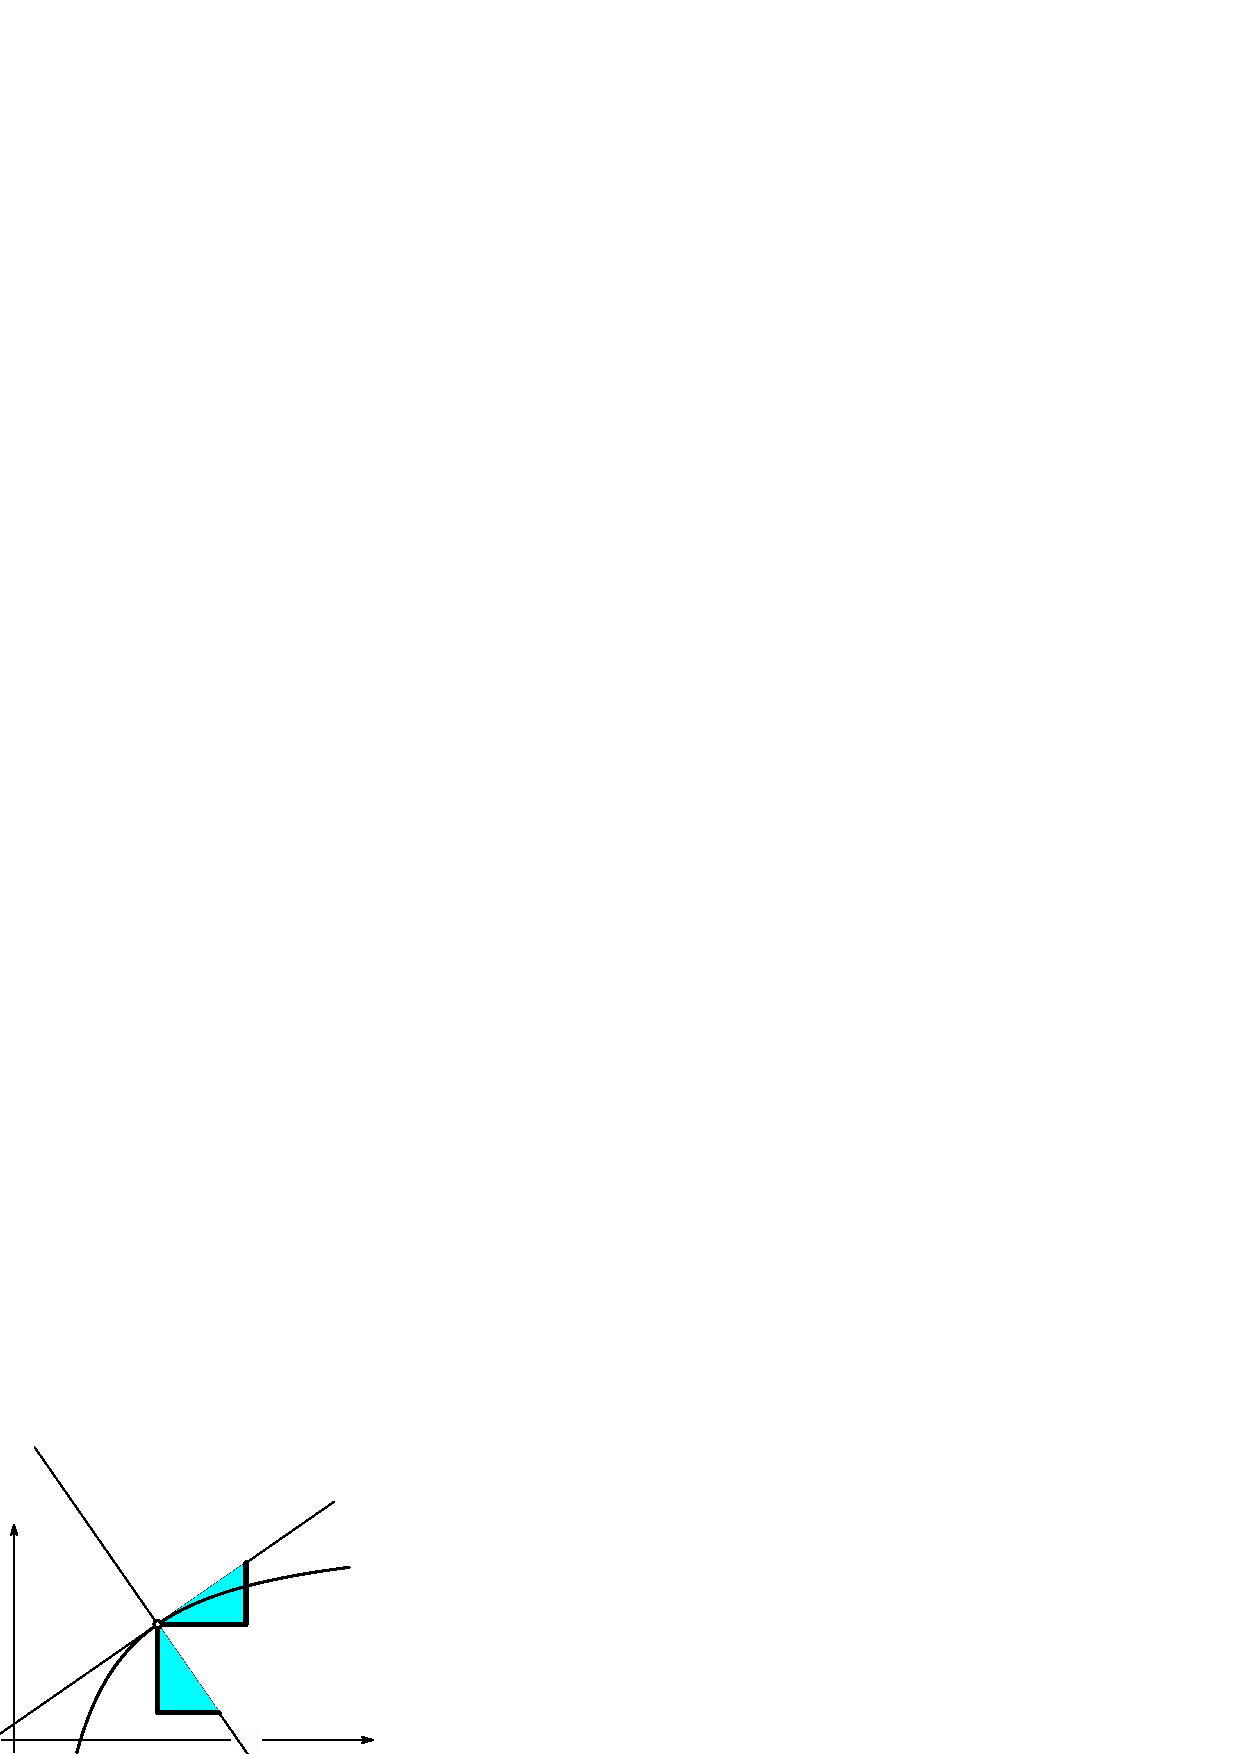
\includegraphics{05tangentAndNormal.pdf}}
        \put(181.00,   4.74){\sffamily\itshape $x$}
    \put(  4.74, 114.10){\sffamily\itshape $y$}
    \put( 60.65,  38.02){\sffamily\itshape $-1$}
    \put( 86.38,  11.80){\sffamily\itshape $m$}
    \put( 94.87,  54.25){\sffamily\itshape $1$}
    \put(120.09,  73.99){\sffamily\itshape $m$}
    \put( 84.62,  74.04){\sffamily\itshape \rotatebox{34.777831}{\footnotesize slope $=m/1=m$}}
    \put( 88.44,  48.27){\sffamily\itshape \rotatebox{-55.222169}{\footnotesize slope $=-1/m$}}
\end{picture}

  \caption{Why ``$\displaystyle \textsf{slope of normal} =
    \frac{-1}{\textsf{slope of tangent}}$.''}
  \label{fig:05tangentAndNormal}
\end{figure}




\section{The Intermediate Value Theorem} %{{{1
  % !!! Discuss: move this section to the "continuity" section.
It is said that a function is continuous if you can draw its graph without
taking your pencil off the paper.  A more precise version of this statement is
the \textit{Intermediate Value Theorem}:




\subsection{Intermediate Value Theorem} %{{{2
\itshape
If $f$ is a continuous function defined on an interval $a\leq x\leq b$, and if $y$ is
any number between $f(a)$ and $f(b)$, then there is a number $c$ with $a\leq
c\leq b$ such that $f(c) = y$.  \upshape\medskip




Here ``$y$ between $f(a)$ and $f(b)$'' means either $f(a)\leq y\leq f(b)$ or $f(b)\leq y\leq f(a)$ depending on which of $f(a)$ or $f(b)$ is larger.




The theorem should be intuitively obvious: to draw the graph you have
to start at $(a, f(a))$ and somehow move your pencil to $(b, f(b))$.
If you do this without taking your pencil off the paper, then at some
point the pencil will have to cross the horizontal line at height $y$
if $y$ is between $f(a)$ and $f(b)$.  That's what the theorem says.




However, this argument is about pencils and paper and it is not about
real numbers and solving equations.  It turns out to be difficult to
give a complete proof of the theorem.  In particular, it requires a
much better description of what a real number is than we are using in
this course.




\begin{figure}\label{fig:05intermediatevalue}
  \centering \input ../figures/221/05intermediatevalue.tex
  \caption{The Intermediate Value Theorem says that a continuous function must
    attain any given value $y$ between $f(a)$ and $f(b)$ at least once.  In this
    example there are three values of $c$ for which $f(c) = y$ holds.}
\end{figure}




\subsection{Example -- Square root of 2} %{{{2
Consider the function $f(x) = x^2$, which we know is continuous. 
Since $f(1)<2$ and $f(2) = 4>2$, the Intermediate Value Theorem with $a=1$,
$b=2$, $y=2$ tells us that there is a number $c$ between $1$ and $2$ such that
$f(c)=2$, i.e.\ for which $c^2=2$.  So the theorem tells us that ``the square
root of $2$ exists''.




\subsection{Example -- The equation $2\theta+\sin\theta=\pi$} %{{{2
    % !!! Issue: It was never proven or even mentioned that sine is continuous!
Consider the function $f(x) = 2x+\sin x$.  It is a continuous function
at all $x$, so from $f(0) = 0$ and $f(\pi) = 2\pi$ it follows that
there is a number $\theta$ between $0$ and $\pi$ such that $f(\theta)
= \pi$.  In other words, the equation
\begin{equation}\label{eq:cplussinc}
  2\theta+\sin \theta =\pi
\end{equation}
has a solution $\theta$ with $0\leq \theta\leq \pi$.  Unlike the
previous example, where we knew the solution was $\sqrt2$, there is no
simple formula for the solution to \eqref{eq:cplussinc}.

\subsection{Example -- ``Solving $1/x=0$''} %{{{2
If we attempt to apply the Intermediate Value Theorem to the function $f(x) =
1/x$ on the interval $[a,b] = [-2, 2]$, then we see that for any $y$
between $f(a) = f(-2) = -\frac12$ and $f(b) = f(2) = \frac12$ there is
a number $c$ in the interval $[-2, 2]$ such that $1/c = y$.  For
instance, we could choose $y=0$ (which lies between $-2$ and $+2$), and
conclude that there is some $c$ with $-2\leq c\leq 2$ and $1/c = 0$.




But there is no such $c$, because $1/c$ is never zero!  So we have done
something wrong: the mistake we made is that we overlooked that our function
$f(x) = 1/x$ is not defined on the \emph{entire} interval $-2\leq x\leq 2$
because it is not defined at $x=0$.  \textit{The moral: always check the
  hypotheses of a theorem before you use it!}
\marginpar{\footnotesize\sffamily%
\input ../figures/221/05intermediatevalue-fail.tex}




\section{Problems} %{{{1
\problemfont %{{{3
\begin{multicols}{2}\setlength{\parindent}{0pt}
\problem Where does the normal line to the graph of $y=x^2$ at the point (1,1) %{{{3
intersect the $x$-axis?
\answer %{{{3
At $x=3$.
\endanswer

\problem Where does the tangent line to the graph of $y=x^2$ at the point $(a, a^2)$ %{{{3
intersect the $x$-axis?
\answer %{{{3
At $x=a/2$.  
\endanswer




\problem Where does the normal line to the graph of $y=x^2$ at the point $(a, a^2)$ %{{{3
intersect the $x$-axis?
\answer %{{{3
At $x=a+2a^3$.  
\endanswer




\problem Find all points on the parabola with the equation $y = x^2 %{{{3
-1$ such that the normal line at the point goes through the origin.




\problem Where does the normal to the graph of $y=\sqrt x$ at the point $(a, %{{{3
\sqrt{a})$
intersect the $x$-axis?
\answer %{{{3
At $x=a+\frac12$.  
\endanswer








\problem Does the graph of $y=x^4-2x^2+2$ have any horizontal tangents?  If %{{{3
so, where? 

Does the graph of the same function have any vertical tangents?

Does it have vertical normals?

Does it have horizontal normals?


\problem At some point $(a, f(a))$ on the graph of $f(x) = -1+2x-x^2$, %{{{3
the tangent to this graph goes through the origin.  Which
point is it?




\problem The line from the origin to the point $(a, f(a))$ on the graph of $f(x) %{{{3
= 1/x^2$ is perpendicular to the tangent line to that graph.  What is $a$?




\problem The line from the origin to the point $(a, f(a))$ on the graph of $f(x) %{{{3
= 4/x$ is perpendicular to the tangent line to the graph.  What is $a$?




\problem Find equations for the tangent and normal lines %{{{3




\textbf{to the curve \ldots} \hfill \textbf{at the point\ldots}\\
\subprob $y=4x/(1+x^2) $ \hfill $(1, 2)$\\
\subprob $y=8/(4+x^2) $ \hfill $(2, 1)$\\
\subprob $y^2=2x+x^2$ \hfill $(2, 2)$\\
\subprob $xy=3$ \hfill $(1, 3)$\\












\problem \groupproblem The function $$f(x) = \frac{x^2+|x|}{x}$$ satisfies $f(-1) = %{{{3
-2$ and $f(+1) = +2$, so, by the Intermediate Value Theorem,
there should be some value $c$ between $-1$ and $+1$ such that
$f(c) = 0$.  \emph{True or False?}
\answer %{{{3
False.  If you try to solve $f(x) = 0$, then you get the equation
$\frac{x^2+|x|}{x}=0$.  If $x\ne0$ then this is the same as
$x^2+|x|=0$, which has no solutions (both terms are positive when
$x\ne0$).  If $x=0$ then $f(x)$ isn't even defined.
So there is no solution to $f(x) = 0$.




This doesn't contradict the IVT, because the function isn't
continuous, in fact it isn't even defined at $x=0$, so the IVT
doesn't have to apply.  
\endanswer


\problem Find the equation for the tangents to the graph of the Backward Sine %{{{3
\[
  f(x)=\sin\left(\dfrac{\pi}{x}\right)
\]
at the points $x=1$, $x=\frac12$ and at $D$  (see Figure \ref{fig:03sinePiOverx}
in \S\ref{sec:03backward-sine}.)




\problem Find the equation for the tangent to the graph of the Backward Cosine %{{{3
in a Bow Tie $g(x)=x\cos\left(\dfrac{\pi}{x}\right)$ at the point $C$  (see Figure
\ref{fig:03backwardCosSandwich} in \S\ref{sec:03xcos1overx})
\end{multicols}




\noproblemfont

\section{Finding sign changes of a function}\label{sec:sign-changes} %{{{1
The Intermediate Value Theorem implies the following very useful fact.

\subsection{Theorem} %{{{2
\label{thm:nosignchangebetweenzeros}\itshape
If $f$ is a continuous function on an interval $a\leq x\leq b$, and if
$f(x)\neq0$ for all $x$ in this interval, then $f(x)$ does not change
its sign in the interval $a\leq x\leq b$: either $f(x)$ is
positive for all $a\leq x\leq b$, or it is negative for all $a\leq x\leq b$.
\upshape




\begin{proof}
  The theorem says that there cannot be two numbers $a \leq x_1<x_2 \leq b$ such
  that $f(x_1)$ and $f(x_2)$ have opposite signs.  If there were two
  such numbers then the Intermediate Value Theorem would imply that
  somewhere between $x_1$ and $x_2$ there would be a $c$ with $f(c)=0$.
  But we are assuming that $f(c)\neq0$ whenever $a \leq c \leq b$. This is a contradiction, so no such $x_1$ and $x_2$ can exist.
\end{proof}




\subsection{Example} %{{{2
Consider
\[
f(x) = (x-3)(x-1)^2(2x+1)^3.
\]
The zeros of $f$ (the solutions of $f(x)=0$) are $ -\frac12, 1, 3 $.
These numbers split the real line into four intervals
\[
(-\infty, -\tfrac12), \quad (-\tfrac12, 1), \quad (1, 3),\quad (3, \infty).
\]
Theorem \ref{thm:nosignchangebetweenzeros} tells us that $f(x)$ cannot change
its sign in any of these intervals.  For instance, $f(x)$ has the same sign for
all $x$ in the first interval $(\infty, -\frac12)$.  Now we choose a number we
like from this interval, say $-1$, and determine that the sign of $f(-1)$:
$f(-1) =(-4)(-2)^2(-1)^3$ is positive.  Therefore $f(x) >0$ for all $x$ in the
interval $(-\infty, -\tfrac12)$.  In the same way we find
\begin{eqnarray*}
  f(-1) = (-4)(-2)^2(-1)^3>0 &\implies & f(x) >0 \text{ for } x<-\tfrac12\\
  f( 0) = (-3)(-1)^2( 1)^3<0 &\implies & f(x) <0 \text{ for } -\tfrac12<x<1\\
  f( 2) = (-1)( 1)^2( 5)^3<0 &\implies & f(x) <0 \text{ for } 1<x<3\\
  f( 4) = ( 1)( 3)^2( 9)^3>0 &\implies & f(x) >0 \text{ for } x>3.
\end{eqnarray*}
If we know all the zeroes of a continuous function, then this method allows us
to decide where the function is positive or negative.  However, when the given
function is factored into easy functions, as in this example, there is a
different way of finding the signs of $f$.  For each of the factors $x-3$,
$(x-1)^2$ and $(2x+1)^3$ it is easy to determine the sign, for any given $x$.
These signs can only change at a zero of the factor.  Thus we have
\begin{itemize}
\item $x-3$ is positive for $x>3$ and negative for $x<3$;
\item $(x-1)^2$ is always positive (except at $x=1$);
\item $(2x+1)^3$ is positive for $x>-\frac12$ and negative for $x<-\frac12$.
\end{itemize}
Multiplying these signs we get the same conclusions as above. We can summarize
this computation in the following diagram:
\begin{figure}[h]
  \centering\sffamily
  \input{../figures/221/05signs-of-f.pdf_tex}
\end{figure}
















\section{Increasing and decreasing functions} %{{{1
Here are four very similar definitions -- look closely to see how they differ.
\begin{itemize}
\item A function is called \emph{increasing} on an interval if $a<b$ implies
  $f(a)<f(b)$ for all numbers $a$ and $b$ in the interval.

\item A function is called \emph{decreasing} on an interval if $a<b$ implies $f(a)>f(b)$ for
  all numbers $a$ and $b$ in the interval.

\item The function $f $ is called \emph{non-decreasing} on an interval if $a<b$ implies
  $f(a)\leq f(b)$ for all numbers $a$ and $b$ in the interval.




\item The function $f $ is called \emph{non-increasing} on an interval if $a<b$ implies
  $f(a)\geq f(b)$ for all numbers $a$ and $b$ in the interval.
\end{itemize}
We can summarize these definitions as follows:
\begin{align*}
 on an interval, \textbf{$f$ is \ldots}\quad\quad&
                           \textbf{if for all $a$ and $b$ in the interval\ldots}\\
  \text{Increasing:}\quad & a<b \implies f(a)<f(b) \\
  \text{Decreasing:}\quad & a<b \implies f(a)>f(b) \\
  \text{Non-increasing:}\quad & a<b \implies f(a)\geq f(b) \\
  \text{Non-decreasing:}\quad & a<b \implies f(a)\leq f(b)
\end{align*}




The definitions of increasing, decreasing, non-increasing, and non-decreasing do
not seem like they are easy to check for a particular function.  But, in fact,
there is an easy test for whether a function is increasing or decreasing: look
at the sign of the derivative of $f$.  More precisely:




\subsection{Theorem}\label{thm:increasing-implies-deriv-pos} %{{{2
\itshape If a differentiable function is non-decreasing on an interval then
$f'(x)\geq 0$ for all $x$ in that interval.

If a differentiable function is non-increasing on an interval then $f'(x)\leq 0$
for all $x$ in that interval.  \upshape

The idea of the proof is the following: if $f$ is non-decreasing, then for any given $x$ and any positive
$\Delta x$, we have $f(x+ \Delta x)\geq f(x)$, so
\[
\frac{f(x+ \Delta x)-f(x)}{\Delta x} \geq 0.
\]
Now if we let $\Delta x\searrow 0$, we see
\[
f'(x) = \lim_{\Delta x\searrow0}\frac{f(x+ \Delta x)-f(x)}{\Delta x} \geq 0.
\]


What about the converse?  In other words, if we know the sign of $f'$ then what can we
say about $f$?  For this we have the following
\subsection{Theorem} %{{{2
\label{thm:deriv-pos-implies-increasing}\itshape
Suppose $f$ is a differentiable function on an interval $(a,b)$.

If $f'(x)>0$ for all $a<x<b$, then $f$ is increasing on the interval.

If $f'(x)<0$ for all $a<x<b$, then $f$ is decreasing on the interval.\upshape
\medskip




The proof is based on the Mean Value Theorem, which also finds use in
many other situations:
\subsection{The Mean Value Theorem} %{{{2
  % !!! Discuss: What is the point of proving the first derivative test via the MVT, without even explaining the MVT or its proof??
\itshape
If $f$ is a differentiable function on the interval $a\leq x\leq b$,
then there is some number $c$ with $a<c<b$ such that
\[
f'(c) = \frac{f(b)-f(a)}{b-a}.
\]
\upshape




\begin{figure}[t]\flushleft\sffamily



  \color{darkbluegreen}
  \parbox[b]{0.45\textwidth}{\textbf{The Mean Value Theorem }says that
    if you pick any two points $A$ and $B$ on the graph of a differentiable function,
    then there always is a point on the graph between $A$ and $B$
    where the tangent line to the graph is parallel to the line segment
    $AB$.  Depending on the shape of the graph and the location of the
    points $A$, $B$, there may even be more than one such point (there are two
    in this figure).  The MVT is used in the proofs of many facts
    about functions; for instance,
    Theorem~\ref{thm:deriv-pos-implies-increasing}.  Here is a picture
  proof of the Mean Value Theorem:}
  \hfill
  \parbox[b]{0.4\textwidth}{\input ../figures/221/05mvt2.tex }




  \def\mvtprooftextone{%
    \parbox[t]{80pt}{\sffamily\itshape\footnotesize\color{darkbluegreen}%
      To find a point on this curve where the tangent is parallel to
      the chord $AB$, you draw two lines \ldots}}




  \def\mvtprooftexttwo{%
    \parbox[b]{96pt}{\sffamily\itshape\footnotesize\color{darkbluegreen}%
      \ldots parallel to the chord, one far above the graph
      and one far below the graph.  Then, always keeping these lines
      parallel to the chord,  you slide them towards the graph \ldots }}




  \def\mvtprooftextthree{%
    \parbox[b]{96pt}{\sffamily\itshape\footnotesize\color{darkbluegreen}%
      \ldots until they touch the
      graph.  At the points where the lines touch the graph, the
      tangent line to the graph is parallel to the chord $AB$. }}
  
  \def\mvtproofthechord{{\sffamily\itshape\footnotesize\color{darkbluegreen} The
  chord $AB$}}

  \input{../figures/221/05mvt-proof.pdf_tex}




  \caption{The Mean Value Theorem}
  \label{fig:05MeanValueTheorem}
  \rule{\textwidth}{2pt}
\end{figure}








\begin{proof}[Proof of theorem \ref{thm:deriv-pos-implies-increasing}]
  We show that $f'(x)>0$ for all $x$ implies that $f$ is increasing.
  (The proof of the other statement is very similar.)
  Let $x_1<x_2$ be two numbers between $a$ and $b$.  Then the Mean Value Theorem
  implies that there is some $c$ between $x_1$ and $x_2$ such that
  \[
  f'(c) = \frac{f(x_2)-f(x_1)}{x_2-x_1},
  \]
  or
  \[
  f(x_2)-f(x_1) = f'(c) (x_2-x_1).
  \]
  Since we know that $f'(c)>0$ and $x_2-x_1>0$ it follows that
  $f(x_2)-f(x_1)>0$, or $f(x_2)>f(x_1)$.
\end{proof}




\section{Examples} %{{{1
Armed with these theorems we can now split the graph of any function into
increasing and decreasing parts simply by computing the derivative $f'(x)$ and
finding out where $f'(x)>0$ and where $f'(x)<0$, and to do this we need only apply the method
  from \ref{sec:sign-changes} to $f'$ rather than $f$.




\subsection{Example: the parabola $y=x^2$} %{{{2
The familiar graph of $f(x)=x^2$ consists of two parts, one decreasing and one
increasing, separated by $x=0$.  You can see this from the derivative which is
\[
f'(x) = 2x
\begin{cases}
  >0 & \text{for $x>0$} \\
  <0 & \text{for $x<0$.}
\end{cases}
\]
Therefore the function $f(x) = x^2$ is \emph{decreasing for $x<0$} and
\emph{increasing for $x>0$.}


% !!! TO-DO: Caption these figures
\begin{figure}[h]
  \centering
  \parbox{170pt}{\input ../figures/221/05parabola.tex}
  \quad
  \parbox{170pt}{\input ../figures/221/05hyperbola.tex}
\end{figure}




\subsection{Example: the hyperbola $ y=1/x $} %{{{2
The derivative of the function $f(x)= 1/x = x^{-1}$ is
\[
f'(x) = -\frac{1}{x^2}
\]
which is always negative.  One might therefore think that this function is
decreasing, or at least non-increasing: if $a<b$ then $1/a \geq 1/b$.  But this
isn't true if we take $a=-1$ and $b=1$:
\[
a=-1<1=b, \text{ but } \frac{1}{a} = -1 < 1 = \frac{1}{b}\text{ !!}
\]
The problem is that we attempted to use theorem
\ref{thm:deriv-pos-implies-increasing}, but this function only applies to
functions \emph{that are defined on an interval}.  The function in this example,
$f(x)=1/x$, is not defined on the interval $-1<x<1$, because it isn't defined at
$x=0$.  That's why we can't conclude that $f(x) = 1/x$ is increasing from $x=-1$
to $x=+1$.




On the other hand, the function is defined and differentiable on the interval
$0<x<\infty$, so theorem \ref{thm:deriv-pos-implies-increasing} tells us that
$f(x) = 1/x$ is decreasing for $x>0$.  This means, that as long as $x$ is
positive, increasing $x$ will decrease $1/x$.




\begin{figure}[t]
  \centering 
    \begin{picture} (270.000000,270.000000)(0,0)
    \put(0.0, 0.0){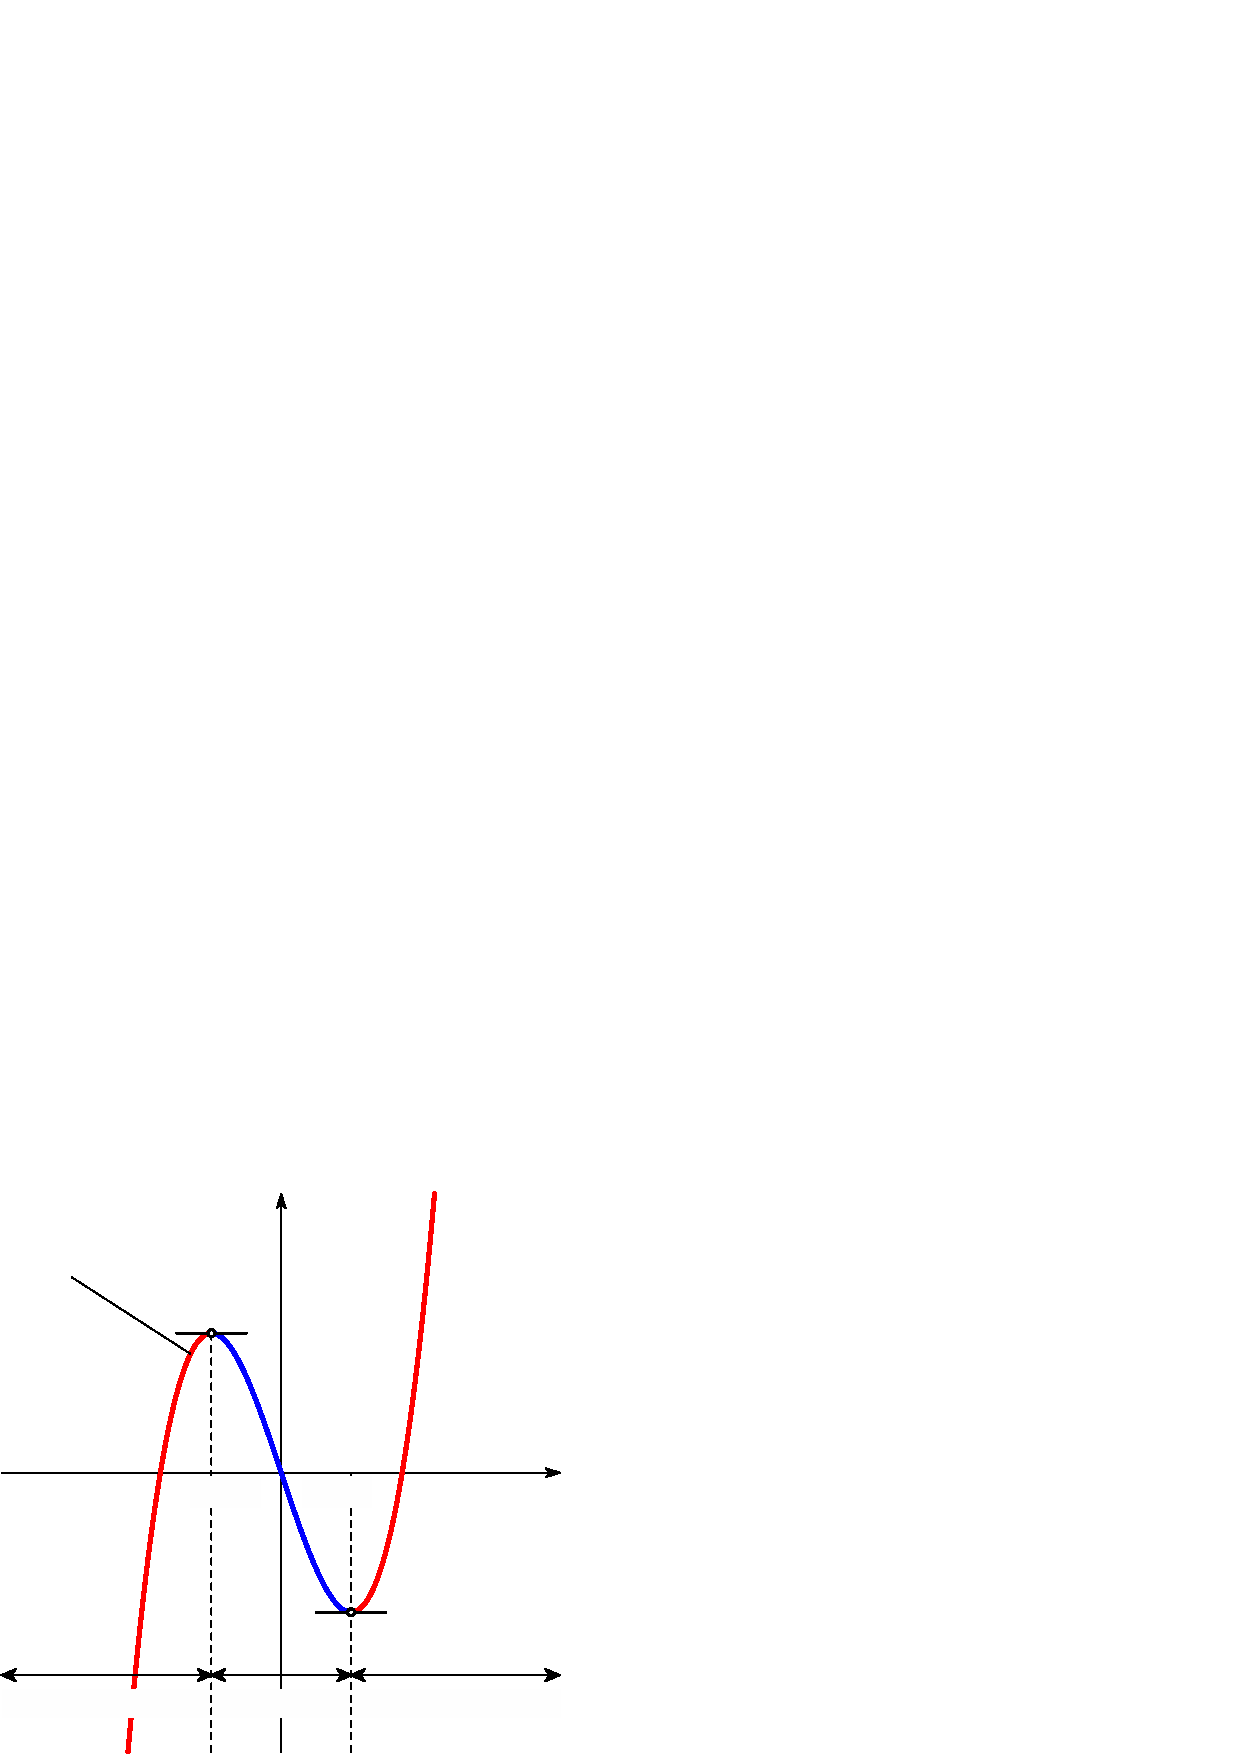
\includegraphics{05upAndDown.pdf}}
        \put( 51.25,  24.50){\sffamily\itshape \makebox[0pt][c]{$f'(x)>0$}}
    \put(218.75,  24.50){\sffamily\itshape \makebox[0pt][c]{$f'(x)>0$}}
    \put(135.00,  24.50){\sffamily\itshape \makebox[0pt][c]{$f'(x)<0$}}
    \put(156.50, 123.00){\sffamily\itshape $x=+1$}
    \put( 89.50, 123.00){\sffamily\itshape $x=-1$}
    \put( 34.50, 235.50){\sffamily\itshape \makebox[0pt][c]{\framebox{$y=x^3-3x$}}}
\end{picture}





  \bigskip




  \caption{The graph of $f(x) = x^3-3x$.}
  \label{fig:05upAndDown}
\end{figure}




\subsection{Graph of a cubic function} %{{{2
\label{sec:cubicgraph}
Consider the function
\[
y = f(x) = x^3-3x.
\]
Its derivative is $f'(x) = 3x^2-3$.  We try to find out where $f'$ is positive,
and where it is negative by factoring $f'(x)$:
\[
f'(x) = 3(x^2-1)
=3(x-1)(x+1)
\]
from which we see that
\begin{align*}
  f'(x) > 0 &\text{ for }x<-1 \\
  f'(x) < 0 &\text{ for }-1 < x < 1 \\
  f'(x) > 0 &\text{ for } x>1
\end{align*}
Therefore the function $f$ is
\begin{center}
  increasing on $(-\infty, -1)$, \quad decreasing on
  $(-1, 1)$, \quad increasing on
  $(1, \infty)$.
\end{center}
At the two points $x=\pm1$ one has $f'(x)=0$ so there the tangent
is horizontal.  This leads to Figure~\ref{fig:05upAndDown}.




\subsection{A function whose tangent turns up and down infinitely often near the origin} %{{{2
We end this section with a weird example.  Somewhere in the mathematician's zoo
of curious functions the following will be on exhibit.  Consider the function
\[
f(x) = \frac x2+x^2\sin\frac\pi x.
\]
(See Figure~\ref{fig:05zigzagBetweenParabolas}.)  For $x=0$ this
formula is undefined so that we still have to define $f(0)$.  We
choose $f(0)=0$.  This makes the function continuous at $x=0$. In
fact, this function is differentiable at $ x=0 $, with derivative
given by
\[
f'(0) = \lim_{x\to 0}\frac{f(x)-f(0)}{x-0} =\lim_{x\to0} \frac12+x\sin\frac\pi
x=\frac12.
\]
(To find the limit, apply the sandwich theorem to $-|x| \leq
x\sin\tfrac\pi x \leq |x|$, as in \S~\ref{sec:backward-cosine-sandwich}.)
\begin{figure}[t]
  \centering 
    \begin{picture} (300.000000,300.000000)(0,0)
    \put(0.0, 0.0){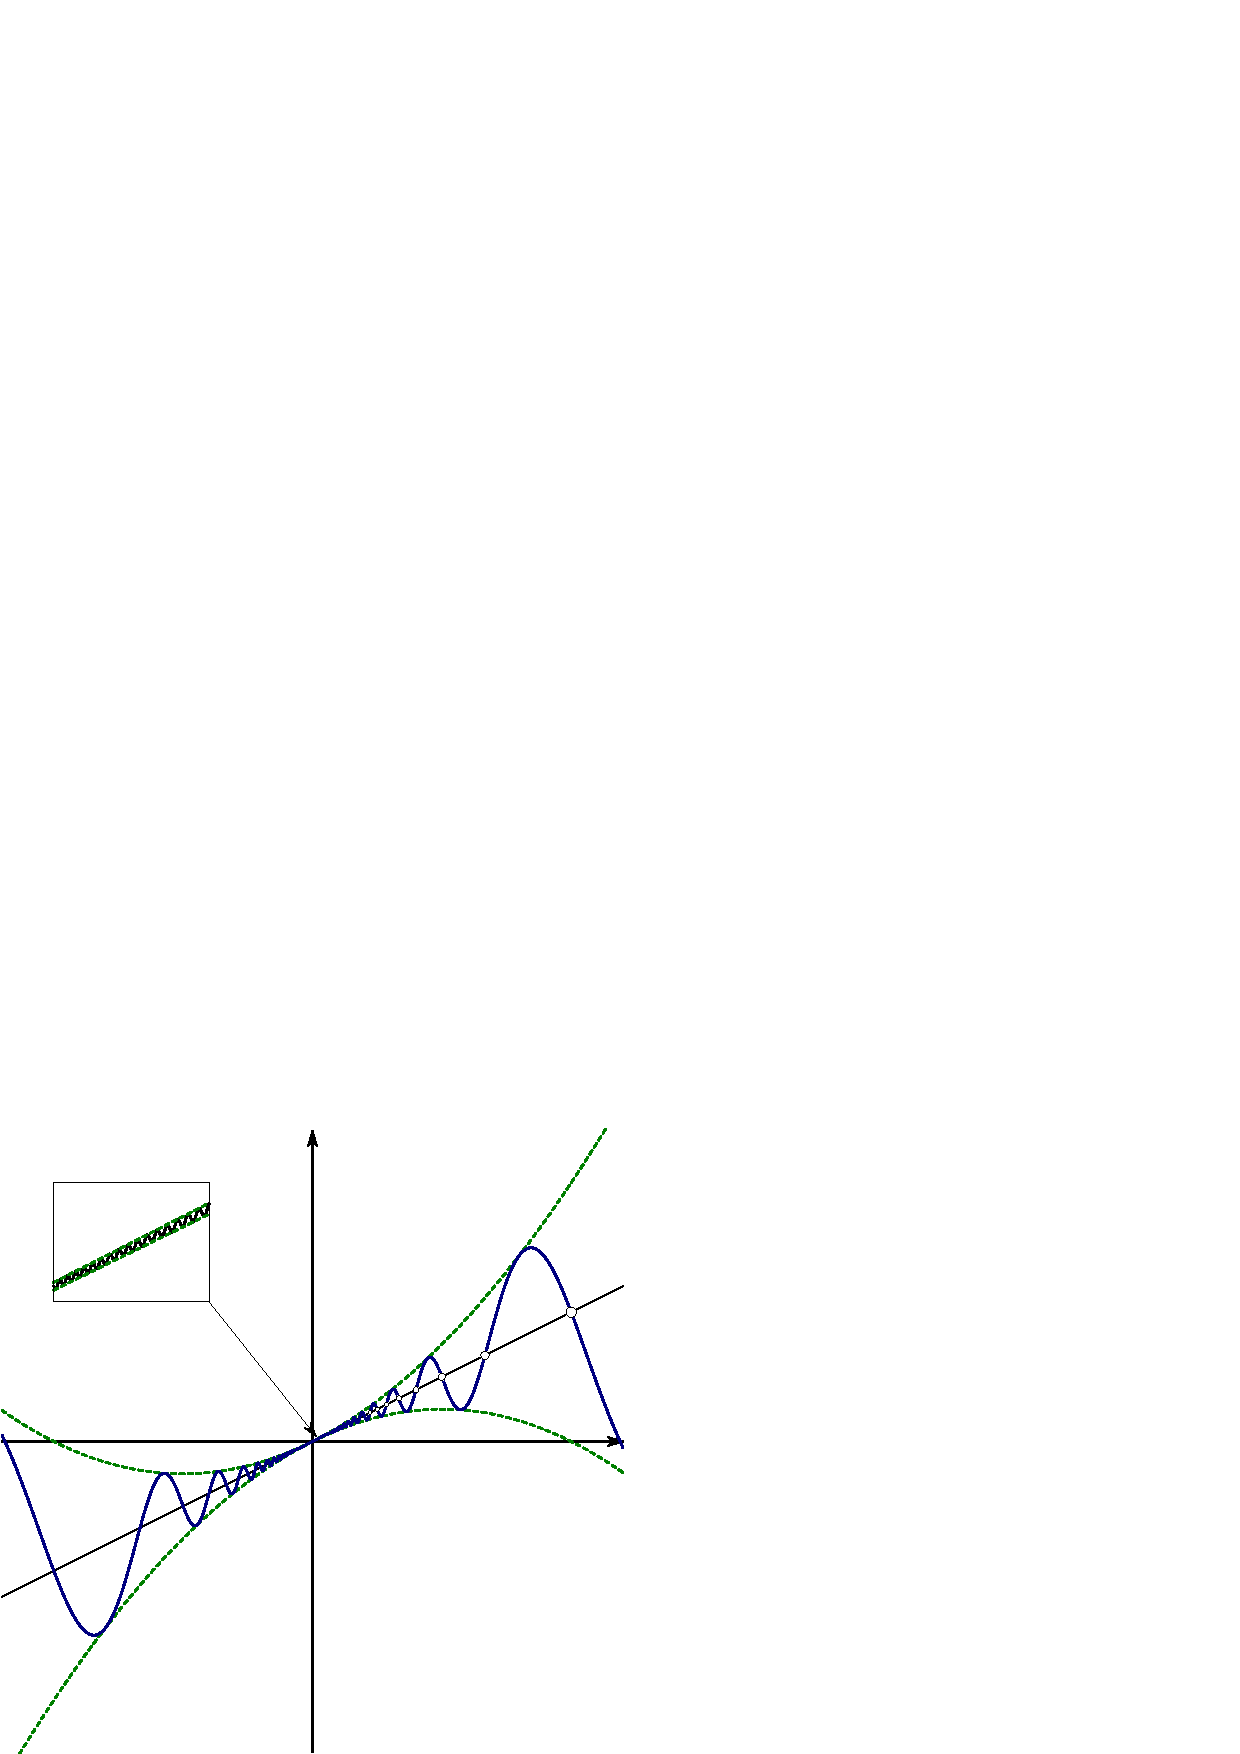
\includegraphics{05zigzagBetweenParabolas2.pdf}}
        \put( 25.83, 207.05){\sffamily\itshape \makebox[0pt][c]{\texttt{\upshape\footnotesize 0.005}}}
    \put(100.33, 207.05){\sffamily\itshape \makebox[0pt][c]{\texttt{\upshape\footnotesize 0.006}}}
    \put( 25.83, 286.17){\sffamily\itshape \makebox[0pt][l]{\parbox{76pt}{\footnotesize\sffamily 
magnification of the graphs near the origin}}}
    \put(278.17, 274.17){\sffamily\itshape $y=\frac 12x+x^2$}
    \put(303.00, 132.10){\sffamily\itshape $y=\frac 12x-x^2$}
    \put(302.00, 224.50){\sffamily\itshape $y=\frac 12x$}
    \put(288.58, 179.68){\sffamily\itshape $y=\frac 12x+x^2\sin\frac\pi x$}
\end{picture}

  \caption{The function $y = \frac12 x+ x^{2}\sin\frac\pi x$ is
    differentiable, and at $x=0$ its derivative is positive (namely,
    $1/2$).  You would think that this means that the function
    therefore has to be increasing near $x=0$, but this example shows
    that the function doesn't have to be increasing near $x=0$.  You
    can see that by zooming in on the graph near the origin.  As you
    follow the graph of $y = \frac12 x+ x^{2}\sin\frac\pi x$ to the
    origin it alternates between increasing and decreasing infinitely
    often.  \label{fig:05zigzagBetweenParabolas}}
\end{figure}




\noindent
The slope of the tangent to the graph at the origin is positive
($\frac12$), and you would \textit{think} that the function should be
``increasing near $x=0$'' But this turns out not to be true!

To see why not, compute the derivative of this function for
$x\neq0$:
\[
f'(x) = \frac12-\pi\cos\frac\pi x+2x\sin\frac\pi x.
\]
We could try to find where $f'(x)$ is positive, and where it's negative, just as
we did for $y=x^3-3x$ in \S~\ref{sec:cubicgraph}, but for this function solving
$f'(x)=0$ turns out to be pretty much impossible.  Fortunately, even though we
can't solve $f'(x) = 0$, we can still find out something about the derivative by
looking at the intersection points of the graph with the line $y=x/2$ and
checking the sign of $f'(x)$ at those points.  We will find that $f'(x)$
flip-flops infinitely often between positive and negative as $x \searrow 0$.  




There are infinitely many intersection points of $y=f(x)$ with $y=x/2$ and the coordinates are
\[
x_k= \frac1k,\quad y_k= f(x_k).
\]
For larger and larger $k$ the points $(x_k, y_k)$ tend to the origin (the $x$
coordinate is $\frac1k$ which goes to 0 as $k\to\infty$).  The slope of the
tangent at $x=x_k$ is given by
\begin{align*}
  f'(x_k) &= \frac12-\pi\cos\frac\pi{1/k} +2\frac1k\sin\frac\pi{1/k}\\
  &= \frac12-\pi \underbrace{\cos k\pi}_{=(-1)^k} +\frac2k
  \underbrace{\sin k\pi}_{=0}\\
  &=\begin{cases}
    \frac12-\pi<0 & \text{for $k$ even}\\[4pt]
    \frac12+\pi>0 & \text{for $k$ odd}
  \end{cases}
\end{align*}
Therefore, along the sequence of points $(x_k, y_k)$ the slope of the tangent
jumps back and forth between $\frac12-\pi$ and $\frac12+\pi$, i.e. between a
positive and a negative number.
In particular, the slope of the tangent at the odd intersection points is
negative, and so you would expect the function to be decreasing there.  
We see that \textit{even though the derivative at $x=0$ of this
particular function is positive, there are points on the graph arbitrarily close
to the origin where the tangent has negative slope.}








\section{Maxima and Minima} %{{{1
A function has a \emph{global maximum} at some $a$ in its domain if $f(x)\leq
f(a)$ for all other $x$ in the domain of $f$.  Global maxima are sometimes also
called ``absolute maxima''.
  
A function has a \emph{global minimum} at some $a$ in its domain if $f(x)\geq
f(a)$ for all other $x$ in the domain of $f$.  Global minima are sometimes also
called ``absolute minima''.




A function has a \emph{local maximum} at some $a$ in its domain if
there is a small $\delta>0$ such that $f(x)\leq f(a)$ for all $x$ with
$a-\delta<x<a+\delta$ that lie in the domain of $f$.
  
A function has a \emph{local minimum} at some $a$ in its domain if
there is a small $\delta>0$ such that $f(x)\leq f(a)$ for all $x$ with
$a-\delta<x<a+\delta$ that lie in the domain of $f$.




Every global maximum is a local maximum, but a local maximum doesn't have to be
a global maximum.
\begin{figure}[h]
  \centering{ 
    \begin{picture} (240.000000,150.750000)(0,0)
    \put(0.0, 0.0){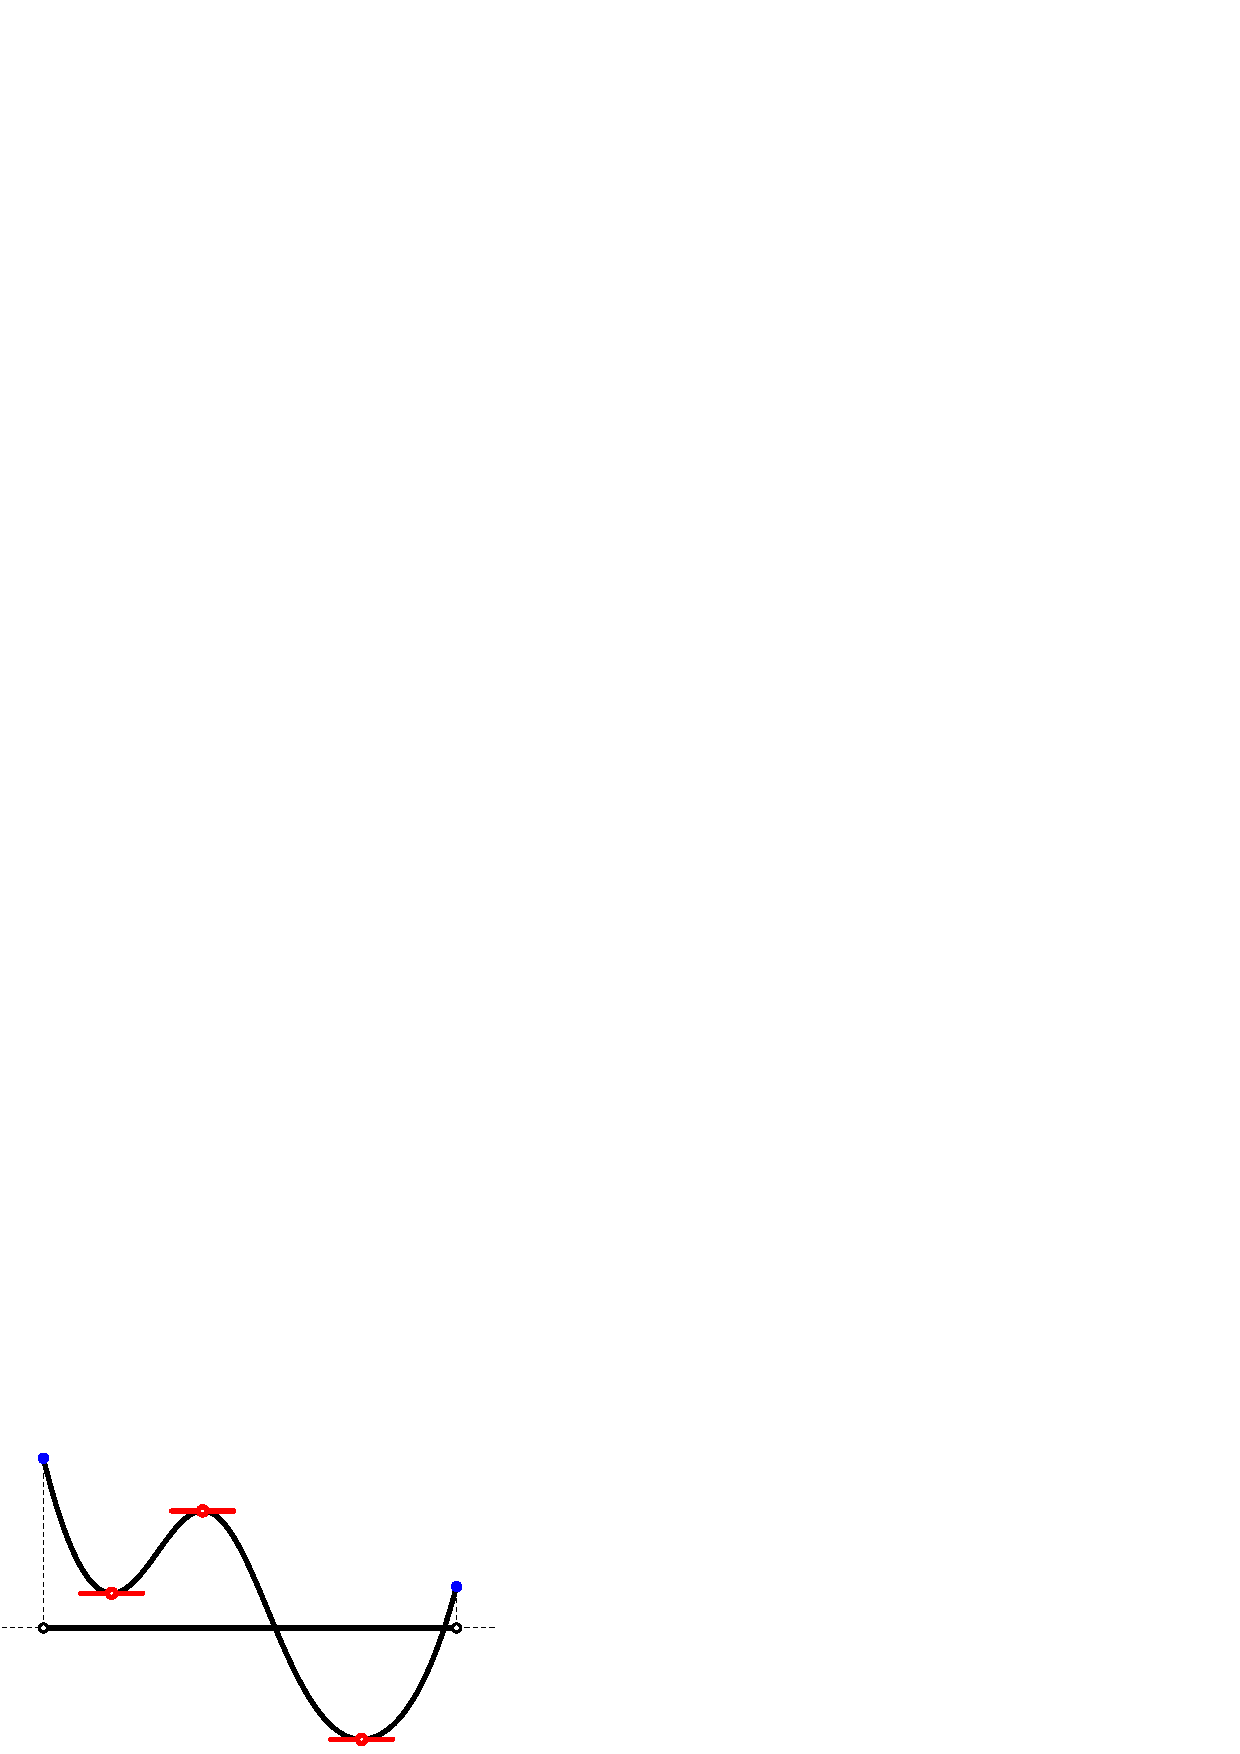
\includegraphics{05minsAndMaxes.pdf}}
        \put( 18.83,  48.50){\sffamily\itshape $a$}
    \put(217.17,  48.50){\sffamily\itshape $b$}
    \put(  8.83, 147.96){\sffamily\itshape {\footnotesize\sffamily\itshape abs max}}
    \put(207.17,  86.35){\sffamily\itshape {\footnotesize\sffamily\itshape loc max}}
    \put( 85.27, 122.67){\sffamily\itshape {\footnotesize\sffamily\itshape loc max}}
    \put( 41.60,  69.18){\sffamily\itshape {\footnotesize\sffamily\itshape loc min}}
    \put(161.59,  -1.01){\sffamily\itshape {\footnotesize\sffamily\itshape abs min}}
\end{picture}
}
  \caption{A function defined on an interval $[a, b]$ with one interior absolute
    minimum, another interior local minimum, an interior local maximum, and two
    local maxima on the boundary, one of which is in fact an absolute maximum.}
  \label{fig:05maxAndMins}
\end{figure}

\subsection{How to find local maxima and minima} %{{{2
\label{sec:where-find-maxes}
Any $x$ value for which $f'(x) = 0$ is called a \emph{stationary point} for the
function $f$.




\begin{theorem}\label{thm:zero-deriv-at-extrema}
  Suppose $f$ is a differentiable function on an interval $[a,b]$.




  Every local maximum or minimum of $f$ is either one of the end points of the
  interval $[a,b]$, or else it is a stationary point for the function $f$.
\end{theorem}




\begin{proof}
  Suppose that $f $ has a local maximum at $x$ and suppose that $x$ is not $a$
  or $b$.  By assumption the left and right hand limits
  \[
  f'(x) = \lim_{\Delta x\nearrow 0}\frac{f(x+\Delta x)-f(x)}{\Delta x} \text{
    and } f'(x) = \lim_{\Delta x\searrow 0}\frac{f(x+\Delta x)-f(x)}{\Delta x}
  \]
  both exist and they are equal.




  Since $f$ has a local maximum at $x$ we have $f(x+\Delta x)-f(x)\leq 0$ if
  $-\delta<\Delta x<\delta$.  In the first limit we also have $\Delta x<0$, so
  that
  \[
  \lim_{\Delta x\nearrow 0}\frac{f(x+\Delta x)-f(x)}{\Delta x} \geq 0.
  \]
  Hence $f'(x) \geq 0$.
% !!! Minor issue: This needs a reference to the limit theorem about inequalities.


  In the second limit we have $\Delta x>0$, so
  \[
  \lim_{\Delta x\searrow 0}\frac{f(x+\Delta x)-f(x)}{\Delta x} \leq 0,
  \]
  which implies $f'(x)\leq 0$.




  Thus we have shown that $f'(x)\leq0$ and $f'(x)\geq 0$ at the same time.  This
  can only be true if $f'(x) = 0$.
\end{proof}




\subsection{How to tell if a stationary point is a maximum, a minimum, or neither} %{{{2
\label{sec:isitamaxormin}
If $f'(c)=0$ then $c$ is a stationary point (by definition), and it might be
local maximum or a local minimum.  You can tell what kind of stationary point
$c$ is by looking at the sign of $f'(x)$ for $x$ near $c$.




\begin{theorem}\label{thm:max-min-test}
  Suppose $y=f(x)$ is function that is defined in an interval
  $(c-\delta, c+\delta)$, where $\delta>0$ is some (small) number.
  \begin{trivlist}
  \item[$\bullet$] If $f'(x)>0$ for $x<c$ and $f'(x)<0$ for $x>c$ then $f$ has a
    local maximum at $x=c$.
  \item[$\bullet$] If $f'(x)<0$ for $x<c$ and $f'(x)>0$ for $x>c$ then $f$ has a
    local minimum at $x=c$.
  \end{trivlist}
\end{theorem}%
\marginpar{\sffamily\itshape\footnotesize%
  \input ../figures/221/05updown-means-max.pdf_tex \\
  \input ../figures/221/05downup-means-min.pdf_tex }
\smallskip




The reason is simple: if $f$ increases to the left of $c$ and decreases to the
right of $c$ then it has a maximum at $c$.  More precisely:




\begin{enumerate}




\item if $f'(x)>0$ for $x$ between $c-\delta$ and $c$, then $f$ is
  increasing for $c-\delta<x<c$ and therefore $f(x)<f(c)$ for $x$
  between $c-\delta$ and $c$.








\item If in addition $f'(x)<0$ for $x>c$ then $f$ is decreasing for
  $x$ between $c$ and $c+\delta$, so that $f(x)<f(c)$ for those $x$.

\item Combining (1) \& (2) gives $f(x)\leq f(c)$ for
  $c-\delta<x<c+\delta$.
\end{enumerate}
The statement about when $f$ has a local minimum follows from an analogous argument.


\subsection{Example -- local maxima and minima of $f(x) = x^3-3x$} %{{{2
\label{sec:locmaxminofcubic}%
In \S\ref{sec:cubicgraph} we found that the function $f(x) =
x^3-3x$ is increasing when $-\infty<x<-1$, and also when $1<x<\infty$,
while it is decreasing when $-1<x<1$.  It follows that the function
has a local maximum at $x=-1$, and a local minimum at $x=1$.

Neither the local maximum nor the local minimum are global since
\[
\lim_{x\to-\infty} f(x) = +\infty\text{ and } \lim_{x\to\infty} f(x) = -\infty.
\]


\subsection{A stationary point that is neither a maximum nor a minimum} %{{{2
If you look for stationary points of the function $f(x) = x^3$ you will find that
there's only one, namely $x=0$.  The derivative $f'(x)=3x^2$ does not change
sign at $x=0$, so the test in Theorem~\ref{thm:max-min-test} does not say
anything.




And in fact, $x=0$ is neither a local maximum nor a local minimum because
$f(x)<f(0)$ for $x<0$ and $f(x)>0$ for $x>0$.
\marginpar{%
  
    \begin{picture} (90.000000,90.000000)(0,0)
    \put(0.0, 0.0){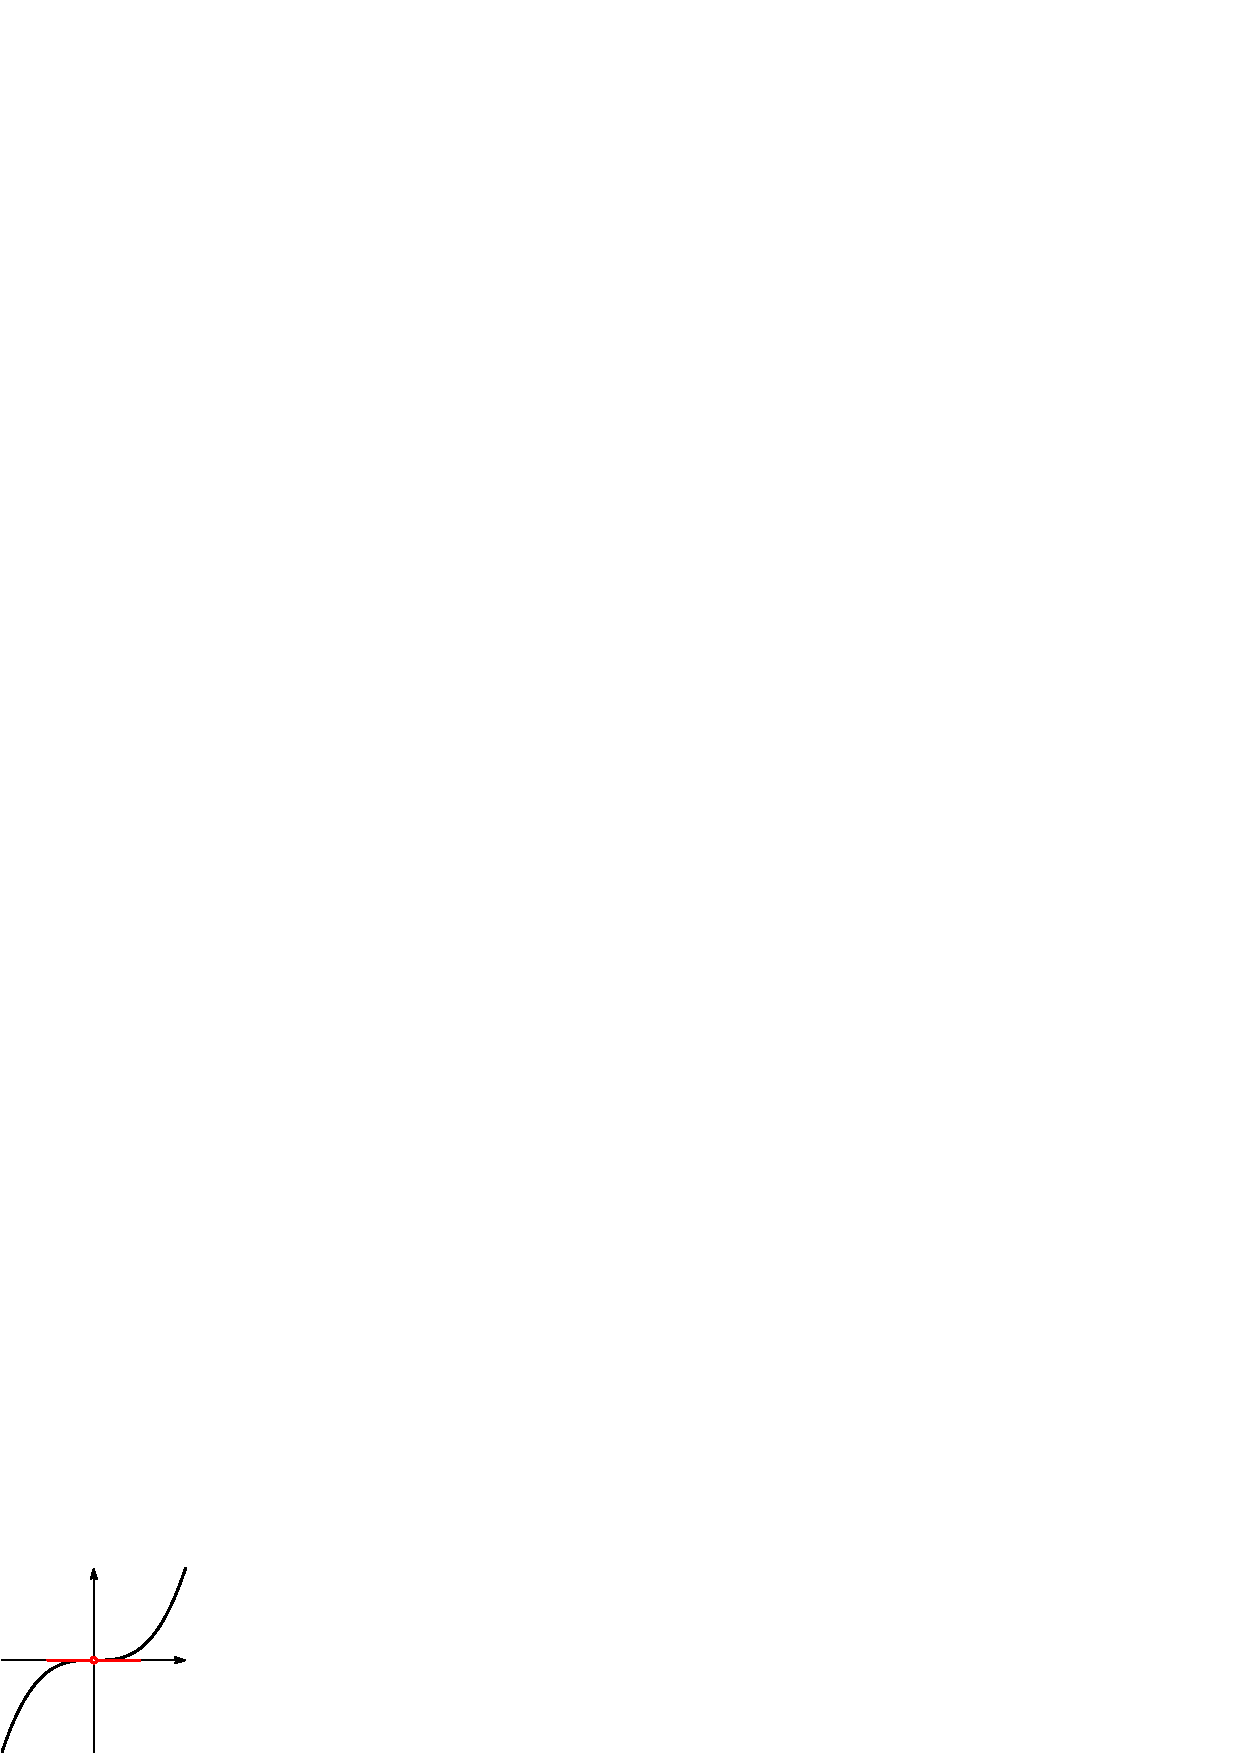
\includegraphics{05neitherMaxNorMin.pdf}}
        \put( 53.80,  80.20){\sffamily\itshape $y=x^3$}
\end{picture}
}

\section{Must a function always have a maximum?} %{{{1
\label{sec:max-exists}
Theorem~\ref{thm:zero-deriv-at-extrema} is very useful since it tells
you how to find (local) maxima and minima.  The following theorem is
also useful, but in a different way.  It doesn't say how to find
maxima or minima, but it tells you that they do exist, and hence that
you are not wasting your time trying to find them.




\begin{theorem}\label{thm:max-min-exist}
  Let $f$ be continuous function defined on the \emph{closed} interval
  $a\leq x\leq b$.  Then $f$ attains its absolute maximum somewhere in this
  interval, and it also attains its absolute minimum somewhere in the interval.
  In other words, there exist real numbers $c$ and $d$ between $a$ and $b$ such that
  \[
  f(c)\leq f(x) \leq f(d)
  \]
  whenever $a\leq x\leq b$.
\end{theorem}\smallskip




This is another one of those theorems whose proof requires a more
careful definition of the real numbers than we have given in Chapter
1.  In this course we will take the theorem for granted.




\section{Examples -- functions with and without maxima or minima} %{{{1
In the following three example we explore what can happen if some of the
hypotheses in Theorem~\ref{thm:max-min-exist} are not met.




\begin{figure}[h]\centering
  \begin{minipage} {110pt}
    
    \begin{picture} (100.000000,93.000000)(0,0)
    \put(0.0, 0.0){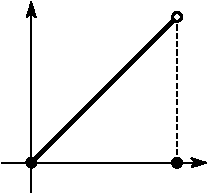
\includegraphics{05xnomax.pdf}}
        \put( 85.00,   3.00){\sffamily\itshape $1$}
    \put( 83.00,  19.00){\sffamily\itshape \makebox[0pt][r]{$f(1)=0$}}
    \put( 13.00,  17.00){\sffamily\itshape \makebox[0pt][r]{min}}
    \put( 90.00,  85.00){\sffamily\itshape \makebox[0pt][l]{max?}}
\end{picture}

  \end{minipage}
  \hfill
  \begin{minipage}{240pt}
    
    \begin{picture} (235.000000,64.730769)(0,0)
    \put(0.0, 0.0){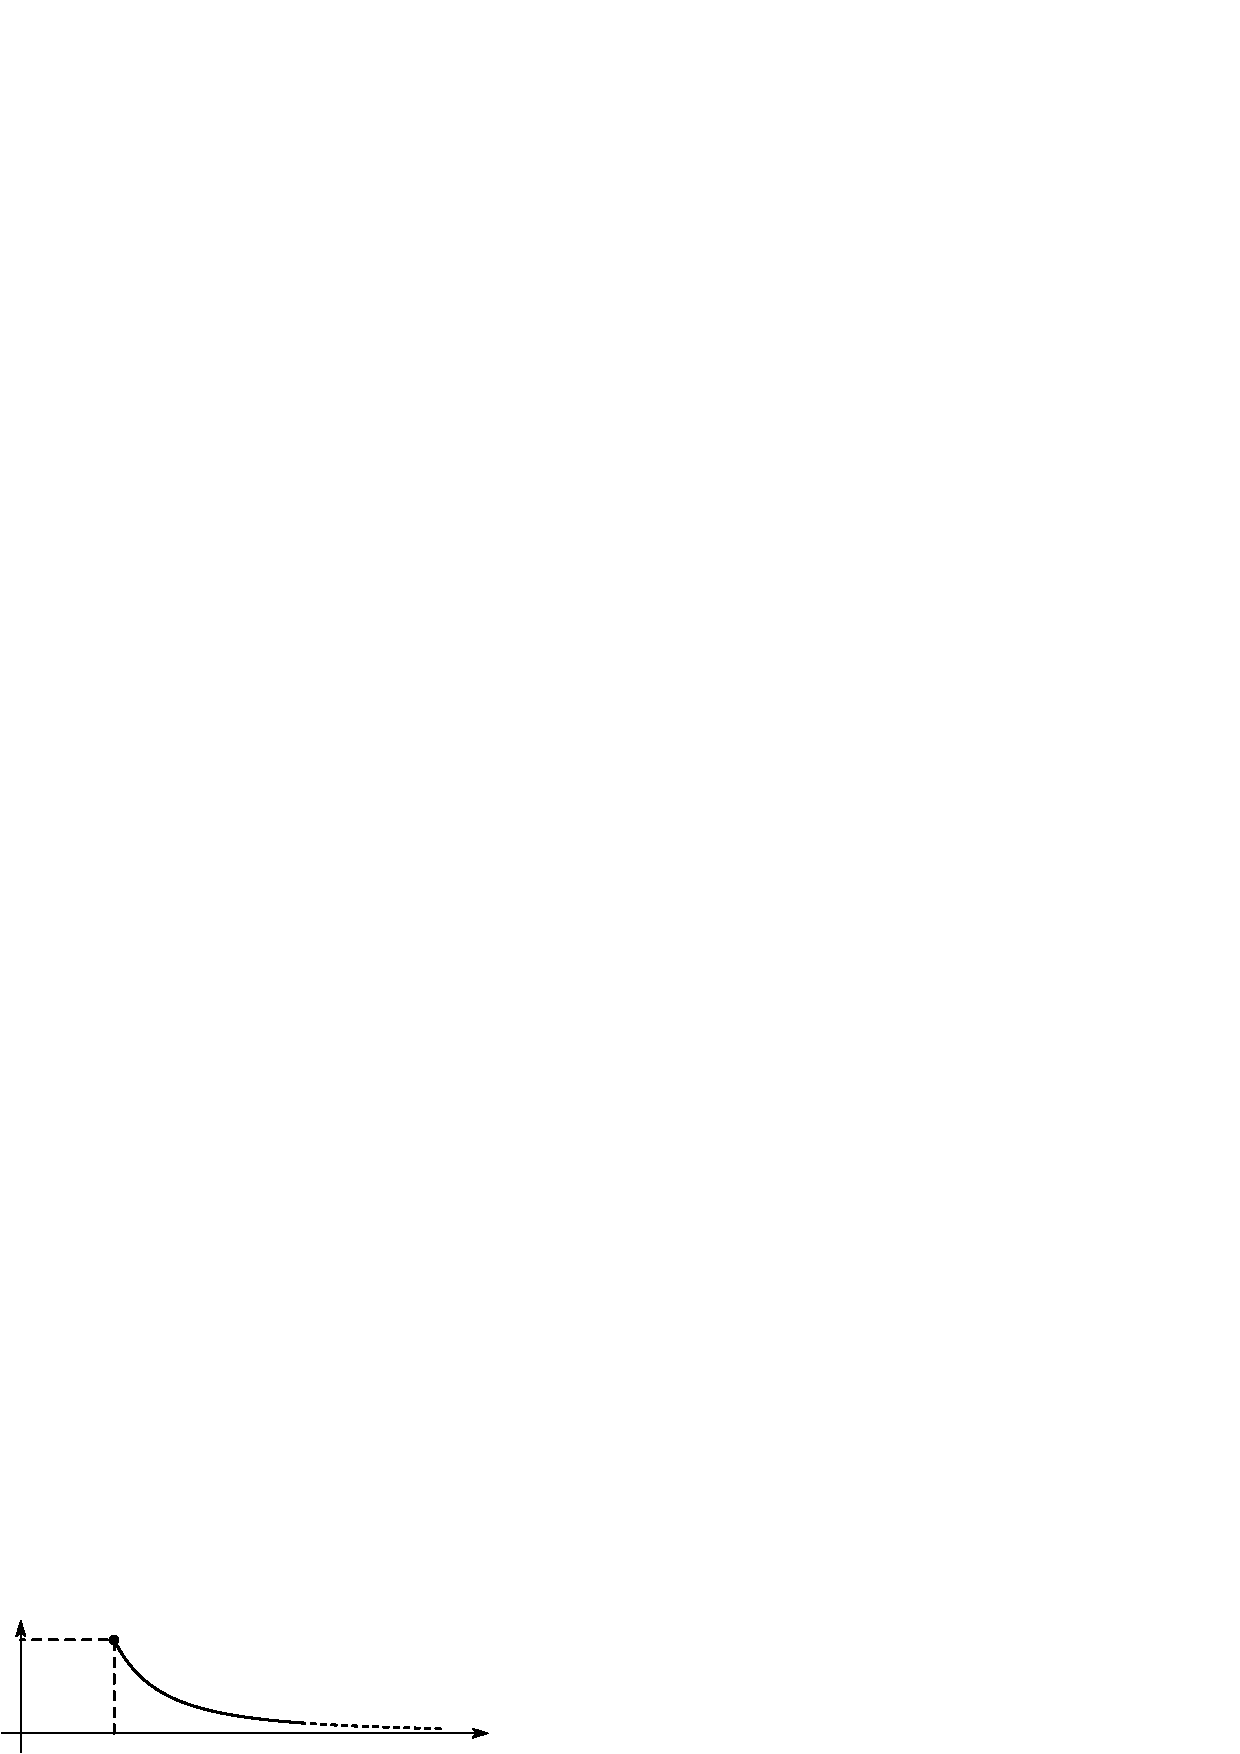
\includegraphics{05xinv_nomin.pdf}}
        \put( 52.77,  -2.04){\sffamily\itshape 1}
    \put( -2.04,  50.77){\sffamily\itshape 1}
    \put( 99.58,  25.16){\sffamily\itshape \makebox[0pt][l]{$y=1/x^2$}}
    \put( 57.77,  58.77){\sffamily\itshape \makebox[0pt][c]{max}}
    \put(211.60,  14.44){\sffamily\itshape \makebox[0pt][c]{min?}}
\end{picture}

  \end{minipage}
  \caption{The function on the left has no maximum, and the one on the right has
    no minimum.}\label{fig:05nomaxnomin}
\end{figure}
\subsection{Question: } %{{{2
\itshape Does the function
\[
f(x) =
\begin{cases}
  x & \text{for }0\leq x<1 \\ 0 &\text{ for }x=1.
\end{cases}
\]
have a maximum on the interval $0\leq x\leq 1$?\upshape




\subsection*{Answer: } %{{{2
No.  What would the maximal value be?  Since
\[
\lim_{x\nearrow1}f(x) = \lim_{x\nearrow1}x = 1,
\]
the maximal value cannot be less than 1.  On the other hand the function is
never larger than $1$.  So if there were a number $a$ in the interval $[0,1]$
such that $f(a)$ was the maximal value of $f$, then we would have to have $f(a) = 1$.
But such an $a$ does not exist!  Conclusion: this function does \emph{not}
attain its maximum on the interval $[0,1]$.




What about Theorem~\ref{thm:max-min-exist}?  That theorem only applies to
continuous functions, and the function $f$ in this example is not continuous at
$x=1$.  It's not continuous because at $x=1$ we have
\[
f(1) = 0, \text{ which is not the same as } \lim_{x\nearrow1} f(x)=1.
\]
So all it takes for Theorem~\ref{thm:max-min-exist} to fail is that
the function $f$ be discontinuous at \textit{just one point}.




\subsection{Question: } %{{{2
\itshape Does the function
\[
f(x) = \frac1{x^2}, \quad 1\leq x<\infty
\]
have a maximum or minimum?\upshape




\subsection*{Answer: } %{{{2
The function has a maximum at $x=1$, but it has no
minimum.




Concerning the maximum: if $x\geq 1$ then $f(x) = 1/{x^2}\leq1$, while
$f(1) = 1$.  Hence $f(x)\leq f(1)$ for all $x$ in the interval $[1,
\infty)$. By definition, this means that $f$ attains its maximum at
$x=1$.








If we look for a minimal value of $f$ then we note that $f(x)\geq0$ for all $x$
in the interval $[1,\infty)$, and also that
\[
\lim_{x\to\infty} f(x) = 0,
\]
so that \emph{if} $f$ attains a minimum at some $a$ with $1\leq a<\infty$, then
the minimal value $f(a)$ must be zero.  However, the equation $f(a) = 0$ has no
solution: $f$ does not attain its minimum.








\subsubsection*{Why did Theorem \ref{thm:max-min-exist} fail this time? }
In this example the function $f$ is continuous on the whole interval
$[1,\infty)$, but this interval is not a closed interval of the
form $[a,b]$.




\section{General method for sketching the graph of a function} %{{{1
  % !!! Issue: Graph-sketching requires concavity information! This section
  % should be moved after the concavity section!
Given a differentiable function $f$ defined on an interval $a\leq x\leq b$,
we can find the increasing and decreasing parts of the graph along with the local maxima and minima by following this procedure:




\begin{enumerate}
\item find all solutions of $f'(x)=0$ in the interval $[a,b]$: these are called
  the \textit{critical} or \textit{stationary} points for $f$.
\item find the sign of $f'(x)$ at all other points
\item each stationary point at which $f'(x)$ actually changes sign is a local
  maximum or local minimum.  Compute the function value $f(x)$ at each
  stationary point.
\item compute the function values at the endpoints of the interval, i.e.\
  compute $f(a)$ and $f(b)$.
\item the absolute maximum is attained at the stationary point or the boundary
  point with the highest function value; the absolute minimum occurs at the
  boundary or stationary point with the smallest function value.
\end{enumerate}
If the interval is unbounded, then instead of computing the values $f(a)$ or
$f(b)$, but instead you should compute $\lim_{x\to\pm\infty}f(x)$.




\subsection{Example -- the graph of a rational function} %{{{2
  % !!! TO-DO: change this function so that the roots of the derivative aren't
  % horrible Remark: If the function is changed to x(3-4x)/(1+x^2) it looks
  % basically identical but the roots of the derivative are much nicer!
Let's sketch the graph of the function
\[
f(x) = \frac{3x(1-x)}{1+x^2}.
\]
By looking at the signs of numerator and denominator we see that
\begin{center}
  $f(x)>0$ for $0<x<1$\\[2pt]
  $f(x)<0$ for $x<0$ and also for $x>1$.
\end{center}
We compute the derivative of $f$:
\[
f'(x) = 3\frac{1-2x-x^2}{\bigl(1+x^2\bigr)^2}.
\]
Hence $f'(x) = 0$ holds if and only if
\[
1-2x-x^2 = 0,
\]
and the solutions to this quadratic equation are $-1\pm\sqrt{2}$.  These two
roots will appear several times and it will shorten our formulas if we
abbreviate
\[
  A= -1 - \sqrt{2} \text{ and } B= -1+\sqrt{2} .
\]

To see if the derivative changes sign we factor the numerator and denominator.
The denominator is always positive, and the numerator is
\[
-x^2-2x+1 = -(x^2+2x-1) =-(x-A)(x-B).
\]
Therefore
\[
f'(x)
\begin{cases}
  <0 & \text{for }x<A \\
  >0 &\text{for } A<x<B \\
  <0 &\text{for } x>B
\end{cases}
\]\marginpar{\sffamily\footnotesize%
\input ../figures/221/05rationalfunction-slopes.pdf_tex}%
It follows that $f$ is decreasing on the interval $(-\infty, A)$, increasing on
the interval $(A, B)$ and decreasing again on the interval $(B, \infty)$.
Therefore
\begin{center}
  $A$ is a local minimum, and $B$ is a local maximum.
\end{center}
Are these global maxima and minima?

\begin{figure}[h]
  \centering 
    \begin{picture} (360.000000,112.809524)(0,0)
    \put(0.0, 0.0){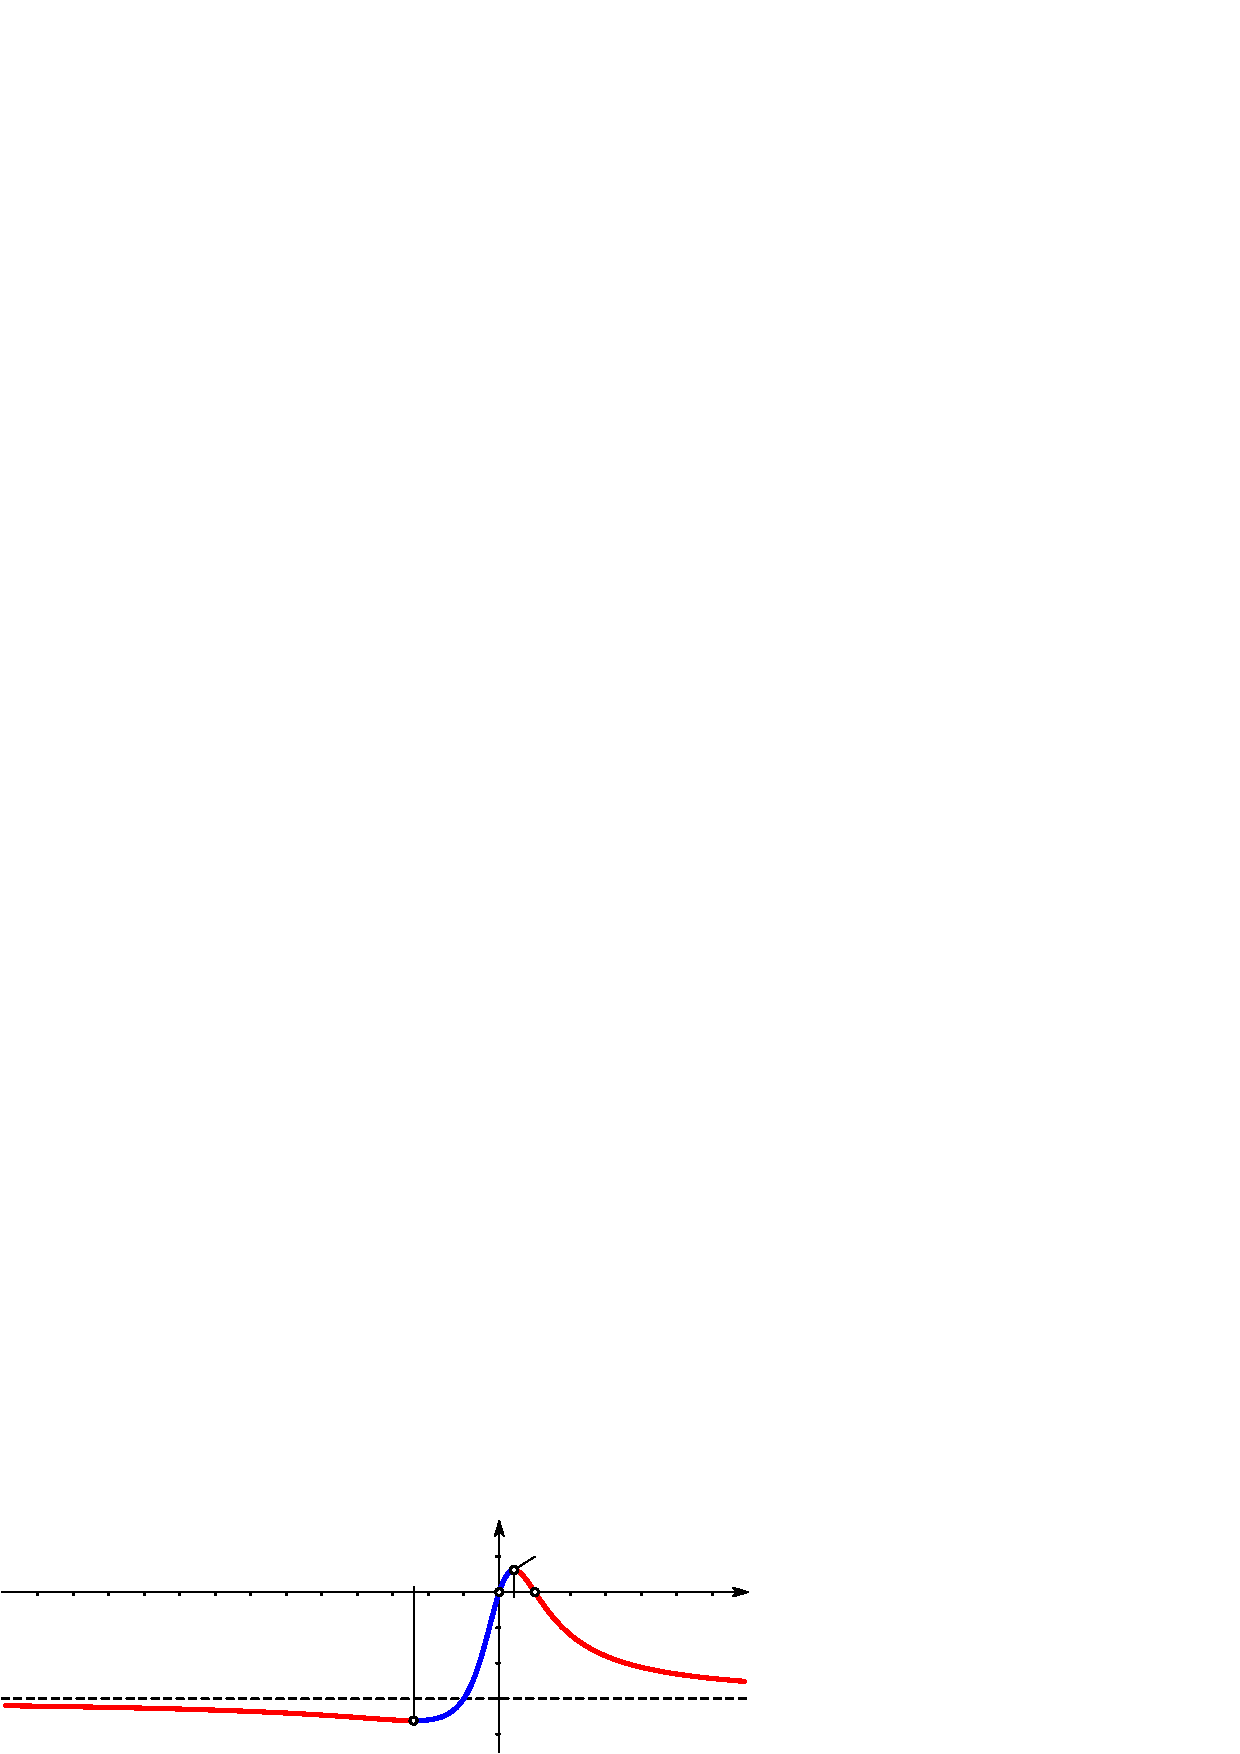
\includegraphics{05rationalexample.pdf}}
        \put( 18.05,  79.71){\sffamily\itshape \makebox[0pt][l]{{\tiny\sffamily\upshape -13}}}
    \put( 35.10,  79.71){\sffamily\itshape \makebox[0pt][l]{{\tiny\sffamily\upshape -12}}}
    \put( 52.14,  79.71){\sffamily\itshape \makebox[0pt][l]{{\tiny\sffamily\upshape -11}}}
    \put( 69.19,  79.71){\sffamily\itshape \makebox[0pt][l]{{\tiny\sffamily\upshape -10}}}
    \put( 86.24,  79.71){\sffamily\itshape \makebox[0pt][l]{{\tiny\sffamily\upshape -9}}}
    \put(103.29,  79.71){\sffamily\itshape \makebox[0pt][l]{{\tiny\sffamily\upshape -8}}}
    \put(120.33,  79.71){\sffamily\itshape \makebox[0pt][l]{{\tiny\sffamily\upshape -7}}}
    \put(137.38,  79.71){\sffamily\itshape \makebox[0pt][l]{{\tiny\sffamily\upshape -6}}}
    \put(154.43,  79.71){\sffamily\itshape \makebox[0pt][l]{{\tiny\sffamily\upshape -5}}}
    \put(171.48,  79.71){\sffamily\itshape \makebox[0pt][l]{{\tiny\sffamily\upshape -4}}}
    \put(188.52,  79.71){\sffamily\itshape \makebox[0pt][l]{{\tiny\sffamily\upshape -3}}}
    \put(205.57,  79.71){\sffamily\itshape \makebox[0pt][l]{{\tiny\sffamily\upshape -2}}}
    \put(222.62,  79.71){\sffamily\itshape \makebox[0pt][l]{{\tiny\sffamily\upshape -1}}}
    \put(256.71,  79.71){\sffamily\itshape \makebox[0pt][l]{{\tiny\sffamily\upshape 1}}}
    \put(273.76,  79.71){\sffamily\itshape \makebox[0pt][l]{{\tiny\sffamily\upshape 2}}}
    \put(290.81,  79.71){\sffamily\itshape \makebox[0pt][l]{{\tiny\sffamily\upshape 3}}}
    \put(307.86,  79.71){\sffamily\itshape \makebox[0pt][l]{{\tiny\sffamily\upshape 4}}}
    \put(324.90,  79.71){\sffamily\itshape \makebox[0pt][l]{{\tiny\sffamily\upshape 5}}}
    \put(341.95,  79.71){\sffamily\itshape \makebox[0pt][l]{{\tiny\sffamily\upshape 6}}}
    \put(243.67,   9.52){\sffamily\itshape \makebox[0pt][c]{{\tiny\sffamily\upshape -4}}}
    \put(243.67,  26.57){\sffamily\itshape \makebox[0pt][c]{{\tiny\sffamily\upshape -3}}}
    \put(243.67,  43.62){\sffamily\itshape \makebox[0pt][c]{{\tiny\sffamily\upshape -2}}}
    \put(243.67,  60.67){\sffamily\itshape \makebox[0pt][c]{{\tiny\sffamily\upshape -1}}}
    \put(243.67,  94.76){\sffamily\itshape \makebox[0pt][c]{{\tiny\sffamily\upshape 1}}}
    \put(180.51,   3.98){\sffamily\itshape abs.~min.}
    \put(258.71,  96.76){\sffamily\itshape abs.~max.}
    \put(195.51,  79.71){\sffamily\itshape $A$}
    \put(243.73,  67.71){\sffamily\itshape $B$}
\end{picture}

  \caption{The graph of $f(x) = 3(x-x^2)/(1+x^2)$}
  \label{fig:05rationalexample}
\end{figure}

Since we are dealing with an unbounded interval we must compute the limits of
$f(x)$ as $x\to\pm\infty$.  We find
\[
\lim_{x\to\infty} f(x) = \lim_{x\to-\infty} f(x) = -3.
\]
Since $f$ is decreasing between $-\infty$ and $A$, it follows that
\[
f(A) \leq f(x) < - 3 \text{ for } -\infty<x\leq A.
\]
Similarly, $f$ is decreasing from $B$ to $+\infty$, so
\[
-3 < f(x) \leq f(B) \text{ for } B < x<\infty.
\]
Between the two stationary points the function is increasing, so
\[
f(A) \leq f(x) \leq f(B) \text{ for } A\leq x\leq B.
\]
From this it follows that $f(x)$ has a global minimum when $x=A=-1-\sqrt{2}$
and has a global maximum when $x=B=-1+\sqrt{2}$.












\section{Convexity, Concavity and the Second Derivative} %{{{1

\subsection{Definition} %{{{2
\itshape A function $f$ is \emph{convex} on some interval
$a<x<b$ if the derivative $f'(x)$ is \emph{increasing} on that interval.




Likewise, the function is called \emph{concave} for $a<x<b$ if the derivative
$f'(x)$ is \emph{decreasing} on that interval.








\upshape\smallskip




In the following drawings the graph on the left is convex, while
\begin{figure}[h]\centering
  \parbox{115pt}{\input ../figures/221/05increasingtangent.tex }
  \parbox{115pt}{\input ../figures/221/05decreasingtangent.tex }
  \parbox{115pt}{\input ../figures/221/05inflectionpoint.tex }
  \caption{\textbf{Convex, concave and mixed graphs.}}
  \label{fig:05concave-convex-examples}
\end{figure}
the one in the middle is concave, because, going from left to right along either of
these graphs (from $A$ to $B$ to $C$ to $D$), you see that the slope of the
tangent increases on the left graph, and decreases on the middle graph.
The third graph is neither convex nor concave, although it does have one concave
piece and one convex piece.

By our results on increasing and decreasing functions, we know that $f$ is
convex if the derivative of $f'(x)$ is positive. In other words, if $f''(x)>0$
for $a<x<b$, then $f'(x)$ is increasing and therefore, by definition, $f(x)$ is
convex.


\subsection{Theorem (convexity and concavity from the second derivative)} %{{{2
\itshape If $f''(x)$ is positive for $a<x<b$, then the function $f$ is convex on
the interval $a<x<b$.

If $f''(x)$ is negative for $a<x<b$, then the function $f$ is concave on that
interval.\upshape\smallskip



\subsection{Definition} %{{{2
\itshape%
A point on the graph of $f$ where $f''(x)$ changes sign is called an
\emph{inflection point}.\upshape\smallskip

The third graph in Figure~\ref{fig:05concave-convex-examples} shows an inflection
point.

\subsection{The chords of convex graphs} %{{{2
Along the graph of a convex function the slope of the tangent is increasing as
you go from left to right.  After you try to draw a couple of such graphs it
really looks like they should always be ``curved upwards.''   The intuitive
understanding of convex and concave is that convex graphs are curved up, and
concave graphs are curved down.

The phrase ``curved upwards'' turns out to be another one of those expressions
whose mathematical definition is not clear (try explaining it with out waving
your hands.)  The following theorem is an attempt to make a more precise
statement that essentially says the graph is curved upwards.

\subsection*{Theorem} %{{{2
\itshape If a function $f$ is convex on some interval
$a<x<b$ then the chord connecting any two points on the graph lies
above the graph.  \upshape\smallskip


While this theorem is still phrased in terms of the picture, the condition that
``the chord lies above the graph'' can be expressed as an inequality between the
function $f(x)$ itself, and the function whose graph is the chord%
\footnote{The precise statement is: a function is convex on the interval $[a,b]$
if, for any $t$ with $0\leq t\leq 1$, and any $c$ and $d$ with $a\leq c < d\leq
b$, it is true that
\[
f(tc+(1-t)d) \leq t \,f(c) + (1-t)\, f(d).
\]
}.
To prove this theorem requires invoking the Mean Value Theorem.
  


\marginpar{\footnotesize\sffamily\itshape\centering
\input ../figures/221/05convexgraphwithchord.pdf_tex \\
The chord connecting $C$ and $D$ lies above the graph.}




\subsection{Example -- the cubic function $f(x) = x^3-3x$} %{{{2
\label{sec:convexpartofcubic}%
The second derivative of the function $f(x) = x^3-3x$ is
\[
f''(x) = 6x
\]
which is positive for $x>0$ and negative for $x<0$. Hence, in the graph in
\S\ref{sec:cubicgraph}, the origin is an inflection point, and the piece of the
graph where $x>0$ is convex, while the piece where $x<0$ is concave.


\subsection{The Second Derivative Test} %{{{2
In \S\ref{sec:isitamaxormin} we saw how you can tell if a stationary point is a
local maximum or minimum by looking at the sign changes of $f'(x)$.  There is
another way of distinguishing between local maxima and minima which involves
computing the second derivative.
\begin{theorem}
  Suppose $c$ is a stationary point for a function $f$.  If $f''(c)<0$, then $f$
  has a local maximum at $x=c$, and if $f''(c)>0$, then $f$ has a local minimum at $c$.
\end{theorem}\smallskip

The theorem doesn't say anything about what happens when $f''(c) = 0$.  To
determine what happens in that case, one must go back to checking the sign of
the first derivative near the stationary point.




The basic reason why this theorem is true is that if $c$ is a stationary point
with $f''(c)>0$, then we know that $f'(x)$ is increasing near $x=c$. But this is
only possible if $f'(x)<0$ for $x<c$ and $f'(x)>0$ for $x>c$ (in some small
interval around $c$).  This means the function $f$ is decreasing for $x<c$ and
increasing for $x>c$, which means it reaches a local minimum at $x=c$. An
analogous argument applies for the $f''(c)<0$ case.
\marginpar{\sffamily\itshape\footnotesize%
  \input ../figures/221/05concave-means-max.pdf_tex \\
  \input ../figures/221/05convex-means-min.pdf_tex }

\subsection{Example -- $f(x) = x^3-3x$, again} %{{{2
Consider the function $f(x) = x^3-3x$ from \S\ref{sec:cubicgraph} and
\S\ref{sec:convexpartofcubic}.  We found that this function has two
stationary points, at $x=\pm1$.  By looking at the sign of
$f'(x) = 3x^2-3$ we concluded that $x=-1$ is a local maximum while
$x=+1$ is a local minimum.
  
Instead of looking at $f'(x)$, we could also have computed $f''(x)$ at $x=\pm1$
and then applied the Second Derivative Test: since $f''(x) = 6x$, we have
\[
f''(-1) = -6 < 0 \text{ and }
f''(+1) = 6 > 0.
\]
Therefore $f$ has a local maximum at $-1$ and a local minimum at $+1$.




\begin{figure}[h]
  \centering 
    \begin{picture} (280.000000,81.428571)(0,0)
    \put(0.0, 0.0){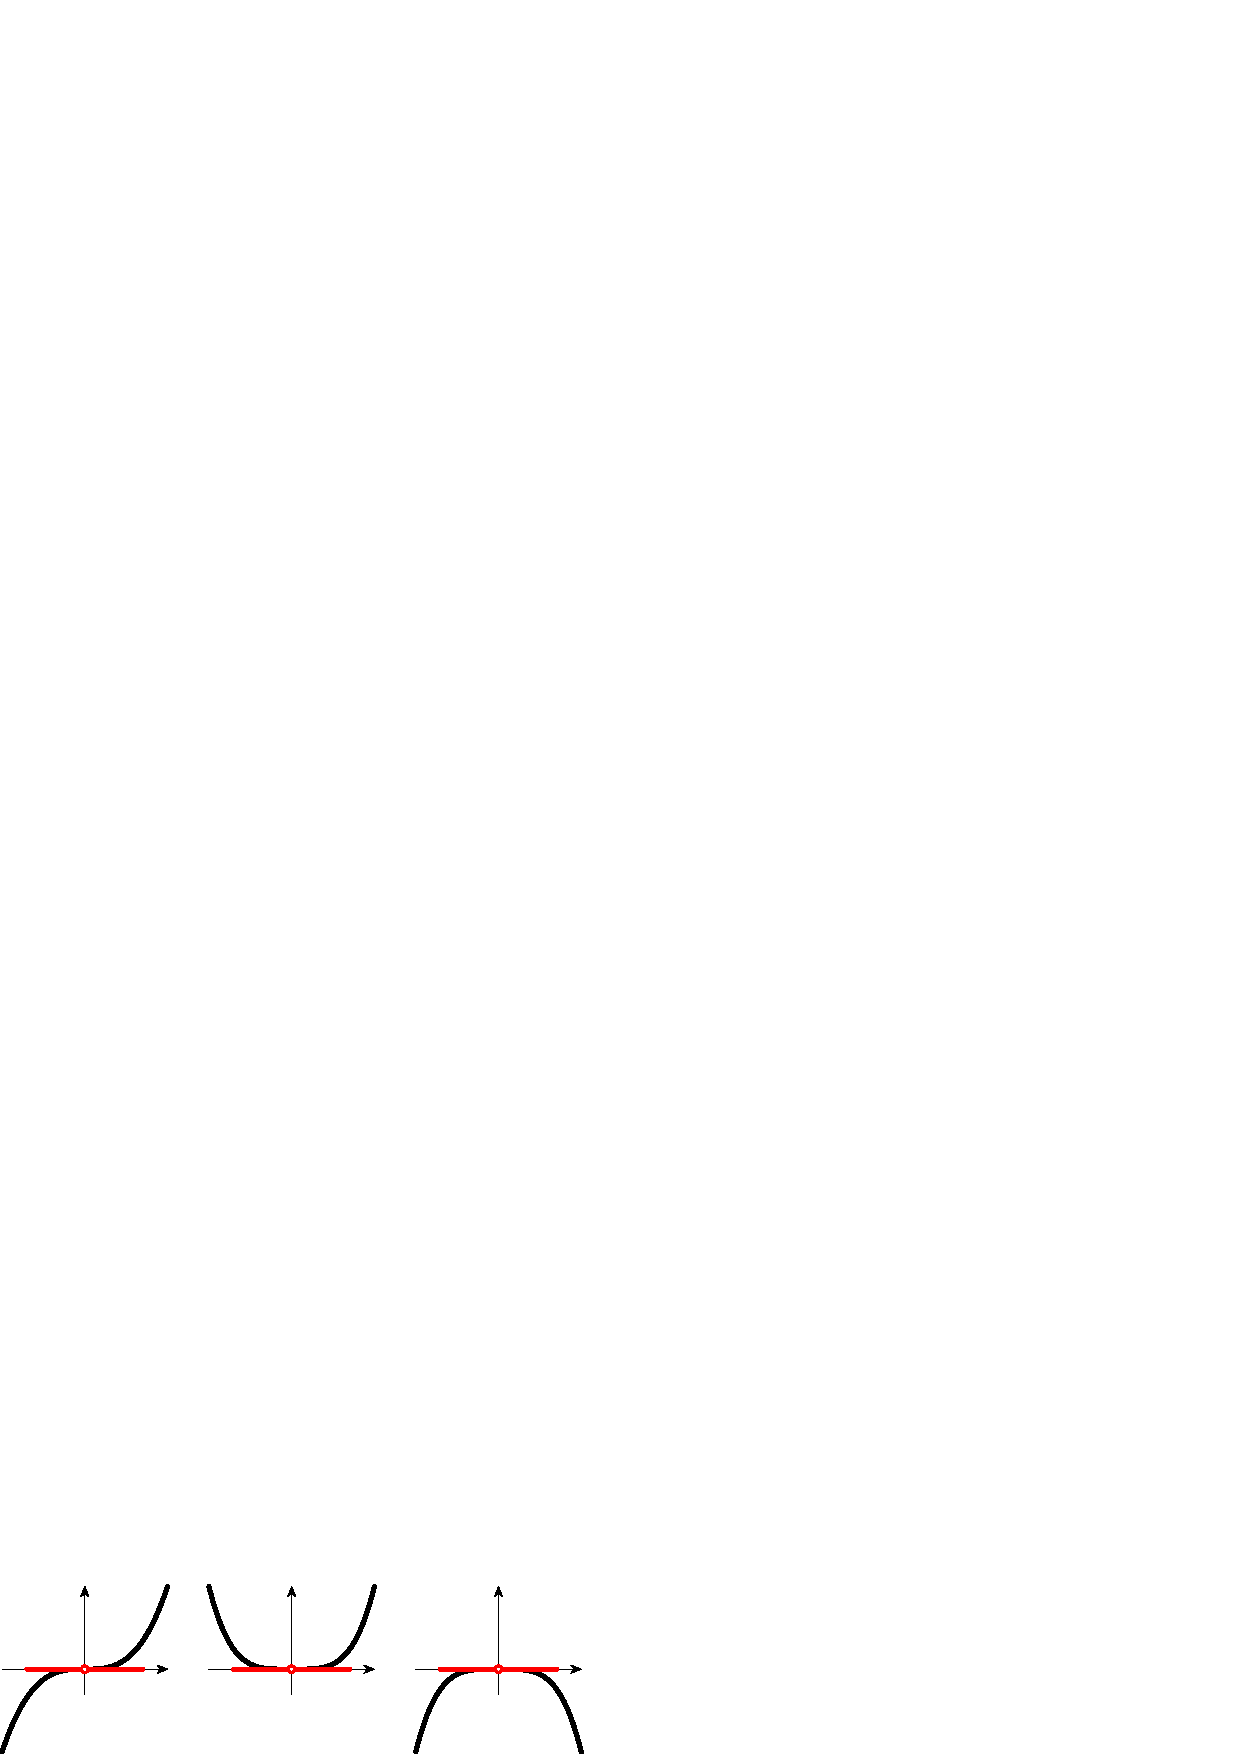
\includegraphics{05nonMorsepoints.pdf}}
        \put( 48.66,  72.49){\sffamily\itshape $y=x^3$}
    \put(147.94,  72.49){\sffamily\itshape $y=x^4$}
    \put(247.23,  72.49){\sffamily\itshape $y=-x^4$}
    \put( 40.71,  16.80){\sffamily\itshape \makebox[0pt][c]{%
\parbox{60pt}{\centering%
neither min\\ nor max}}}
    \put(140.00,  16.80){\sffamily\itshape \makebox[0pt][c]{local min}}
    \put(239.29,  16.80){\sffamily\itshape \makebox[0pt][c]{local max}}
\end{picture}

  \caption{Three functions for which the second derivative test
    doesn't work.}
  \label{fig:05nonMorsepoints}
\end{figure}




\subsection{When the second derivative test doesn't work} %{{{2
Usually the second derivative test will work, but sometimes a
stationary point $c$ has $f''(c)=0$.  In this case the second
derivative test gives no information at all.
Figure~\ref{fig:05nonMorsepoints} shows you the graphs of three
functions, all three of which have a stationary point at $x=0$.  In
all three cases the second derivative vanishes at $x=0$ so the second
derivative test says nothing.  As you can see, the stationary point
can be a local maximum, a local minimum, or neither.








\section{Problems} %{{{1
\problemfont %{{{3
\begin{multicols}{2}\setlength{\parindent}{0pt}




\problem What does the Intermediate Value Theorem say? %{{{3




\problem What does the Mean Value Theorem say? %{{{3

\problem  \textit{Rolle's Theorem} says that there is a stationary %{{{3
point between any pair of zeros of a function.  More precisely,
\begin{center}
  \rmfamily\itshape If $f(a) = 0$ and $f(b)=0$ then there is a $c$
  between $a$ and $b$ such that $f'(c) = 0$.
\end{center}
Show that this follows from the Mean Value Theorem. (Hint: It's a special case
of the Mean Value Theorem.  You can mimic the proof that was given in the text.)


\problem What is a stationary point? %{{{3




\problem \groupproblem How can you tell if a local maximum is a global %{{{3
maximum?




\problem \groupproblem If $f''(a) = 0$ then the graph of $f$ has an %{{{3
inflection point at $x=a$.  \emph{True or False?}
\answer %{{{3
Not necessarily true, and therefore false.  Consider the example
$f(x)=x^4$, and see the next problem.
\endanswer




\problem What is an inflection point? %{{{3
\answer %{{{3
An inflection point is a point on the graph of a function where the
second derivative changes its sign.  At such a point you must have
$f''(x) = 0$, but by itself that it is no enough.
\endanswer




\problem Give an example of a function for which $f'(0)=0$ even though the %{{{3
function $f$ has neither a local maximum or a local minimum at $x=0$.




\problem \groupproblem Draw four graphs of functions, one for each of %{{{3
the following four combinations:
\begin{align*}
  &f'>0\text{ and } f''>0 \\   &f'>0\text{ and } f''<0 \\
  &f'<0\text{ and } f''>0 \\   &f'<0\text{ and } f''<0 \\
\end{align*}

\problem \groupproblem Which of the following combinations are possible? %{{{3
\begin{align*}
  \textbf{(a)~}& f'(x)>0 \text{ and } f''(x)=0 \text{ for all } x \\
  \textbf{(b)~}& f'(x)=0 \text{ and } f''(x)>0 \text{ for all } x
\end{align*}
\answer %{{{3
The first is possible, e.g.~$f(x) = x$ satisfies $f'(x)>0$ and
$f''(x)=0$ for all $x$.

The second is impossible, since $f''$ is the derivative of
$f'$, so $f'(x) = 0$ for all $x$ implies that
$f''(x)=0$ for all $x$.
\endanswer








\bigskip




For each of the following functions, decide if they are
increasing, decreasing, or neither on the indicated intervals:

\problem $\displaystyle f(x) = \frac{x}{1+x^2} \text{, on }  10<x<\infty$ %{{{3

\problem $\displaystyle f(x) = \frac{2+x^2}{x^3-x} \text{, on }  1<x<\infty$ %{{{3

\problem $\displaystyle f(x) = \frac{2+x^2}{x^3-x} \text{, on }  0<x<1$ %{{{3

\problem $\displaystyle f(x) = \frac{2+x^2}{x^3-x} \text{, on }  0<x<\infty$ %{{{3

\bigskip

\textbf{Sketch the graphs} of the following functions.
You should
\begin{list}{--}{
    \setlength{\itemindent}{0pt}
    \setlength{\leftmargin}{6pt}}
\item find where $f$, $f'$ and $f''$ are positive or negative
\item find all stationary points and classify them as local minima, maxima, or neither
\item find any global maxima or minima, if they exist
\item find all inflection points
\item determine all intervals where the function is increasing or decreasing
\item determine all intervals where the function is convex or concave
\item find any horizontal, vertical, or slant asymptotes
\end{list}
















\problem $\displaystyle y=x^3+2x^2 $ %{{{3
\answer %{{{3
$y=0$ at $x=-1, 0, 0$.  Only sign change at $x=-1$, not at $x=0$.

$x=0$ loc min;  $x=-\frac43$ loc max;  $x=-2/3$ inflection point.
No global max or min.
\endanswer




\problem $\displaystyle y=x^3-4x^2$ %{{{3
\answer %{{{3
zero at $x=0, 4$; sign change at $x=4$; loc min at $x=\frac83$; loc
max at $x=0$; inflection point at $x=4/3$.  No global max or min.
\endanswer




\problem $\displaystyle y=x^4+27x $ %{{{3
\answer %{{{3
sign changes at $x=0, -3$;  global min at $x=-3/4^{1/3}$; no inflection
points, the graph is convex.
\endanswer




\problem $\displaystyle y=x^4-27x$ %{{{3
\answer %{{{3
mirror image of previous problem.
\endanswer




\problem $\displaystyle y=x^4+2x^2-3 $ %{{{3
\answer %{{{3
$x^4+2x^2-3 = \bigl(x^2-1\bigr)\bigl(x^2+3\bigr)$ so sign changes at
$x=\pm1$.  Global min at $x=0$;  graph is convex, no inflection points.
\endanswer




\problem $\displaystyle y=x^4-5x^2+4 $ %{{{3
\answer %{{{3
Sign changes at $\pm2, \pm1$;  \emph{two} global minima, at $\pm\sqrt{5/2}$;
one local max at x=0;  two inflection points, at $x=\pm\sqrt{5/6}$.
\endanswer




\problem $\displaystyle y=x^5+16x$ %{{{3
\answer %{{{3
Sign change at $x=0$;  function is always increasing so no stationary
points;  inflection point at $x=0$.
\endanswer




\problem $\displaystyle y=x^5-16x$ %{{{3
\answer %{{{3
sign change at $x=0, \pm 2$;  loc max at $x=2/5^{1/4}$; loc min at
$x=-2/5^{1/4}$. Inflection point at $x=0$.
\endanswer




\problem $\displaystyle y=\frac{x} {x+1}$ %{{{3
\answer %{{{3
Function not defined at $x=-1$.  For $x>-1$ sign change at $x=0$, no
stationary points, no inflection points (graph is concave).
Horizontal asymptote $\lim_{x\to \infty}f(x) = 1$.




For $x<-1$ no sign change , function is increasing and convex, horizontal
asymptote with $\lim_{x\to-\infty}f(x) = 1$.
\endanswer




\problem $\displaystyle y=\frac{x}{1+x^2}$ %{{{3
\answer %{{{3
global max (min) at $x=1$ (x=-1), inflection points at $x=\pm\surd3$;
horizontal asymptotes $\lim_{x\to \pm\infty}f(x) = 0$.
\endanswer




\problem $\displaystyle y=\frac{x^2}{1+x^2}$ %{{{3
\answer %{{{3
$y=0$ at $x=0$ but no sign changes anywhere;  $x=0$ is a global min;
there's no local or global max;  two inflection points at
$x=\pm\frac13\surd3$; horizontal asymptotes at height $y=1$.
\endanswer




\problem $\displaystyle y=\frac{1+x^2}{1+x}$ %{{{3
\answer %{{{3
Not defined at $x=-1$.  For $x>-1$ the graph is convex and has a
minimum at $x=-1+\surd2$;  for $x<-1$ the graph is concave with a
maximum at $x=-1-\surd2$.  No horizontal asymptotes.
\endanswer




\problem $\displaystyle y=x+\frac1x$ %{{{3
\answer %{{{3
Not def'd at $x=0$. No sign changes (except at $x=0$).
For $x>0$ convex with minimum at $x=1$, for $x<0$ concave
with maximum at $x=-1$.
\endanswer




\problem $\displaystyle y=x-\frac1x$ %{{{3
\answer %{{{3
Not def'd at $x=0$. Sign changes at $x=\pm1$ and also at $x=0$.
No stationary points.  Both branches ($x>0$ and $x<0$) are
increasing.  Non inflection points, no horizontal asymptotes.
\endanswer




\problem $\displaystyle y=x^3+2x^2+x$ %{{{3
\answer %{{{3
Zero at $x=0, -1 $ sign only changes at $-1$;  loc min at
$x=-\frac13$; loc max at $x=-1$.  Inflection point at $x=-2/3$.
\endanswer




\problem $\displaystyle y=x^3+2x^2-x$ %{{{3
\answer %{{{3
Changes sign at $x=-1\pm\surd2$ and $x=0$; loc min at
$(-2+\surd7)/3$, loc max at $(-2-\surd7)/3$; inflection point at
$x=-\frac23$.
\endanswer




\problem $\displaystyle y=x^4-x^3-x$ %{{{3
\answer %{{{3
Factor $y=x^4-x^3-x=x(x^3-x^2-1)$.  One zero is obvious, namely
at $x=0$.  For the other(s) you must solve $x^3-x^2-1=0$ which is
beyond what's expected in this course.\\
The derivative is $y'=4x^3-3x^2-1$.  A cubic function whose
coefficients add up to 0 so $x=1$ is a root, and you can factor
$y'=4x^3-3x^2-1= (x-1)(4x^2+x+1)$ from which you see that $x=1$
is the only root.  So: one stationary point at $x=1$, which is a
global minimum\\
The second derivative is $y''=12x^2-6x$; there are two inflection
points, at $x=\frac12$ and at $x=0$.
\endanswer




\problem $\displaystyle y=x^4-2x^3+2x$ %{{{3
\answer %{{{3
Again one obvious solution to $y=0$, namely $x=0$.  The other
require solving a cubic equation.\\ The derivative is
$y'=4x^3-6x^2+2$ which is also cubic, but the coefficients add up to
0, so $x=1$ is a root.  You can then factor
$y'=4x^3-6x^2+2=(x-1)(4x^2-2x-2)$.  There are three stationary
points: local minima at $x=1$, $x=-\frac14 - \frac12\surd3$, local
max at $x=-\frac14 + \frac12\surd3$.  One of the two loc min is a
global minimum.
\endanswer




\problem $\displaystyle y=\sqrt{1+x^2}$ %{{{3
\answer %{{{3
Global min at $x=0$, no other stationary points;  function is
convex, no inflection points.  No horizontal asymptotes.
\endanswer




\problem $\displaystyle y=\sqrt{1-x^2}$ %{{{3
\answer %{{{3
The graph is the upper half of the unit circle.
\endanswer




\problem $\displaystyle y=\sqrt[4]{1+x^2}$ %{{{3
\answer %{{{3
Always positive, so no sign changes;  global minimum at $x=0$, no
other stationary points; two inflection points at $\pm\surd2$.  No
horizontal asymptotes since $\lim_{x\to\pm\infty} \sqrt[4]{1+x^2} =
\infty \textrm{(DNE)}$.
\endanswer




\problem $\displaystyle y=\frac1{1+x^4} $ %{{{3
\answer %{{{3
Always positive hence no sign changes; global max at $x=0$, no other
stationary points;  two inflection points at $x=\pm\sqrt[4]{3/5}$;
second derivative also vanishes at $x=0$ but this is not an
inflection point.
\endanswer








\bigskip
\noindent%
The following functions are \textbf{periodic}, meaning that they satisfy $f(x+L)=f(x)$ for
  all $x$ and a constant $L$ called the \textbf{period} of the function.  The
graph of a periodic function repeats itself indefinitely to the left and to
the right.  It therefore has infinitely many (local) minima and maxima, and
infinitely many inflection points.  Sketch the graphs of the following
functions as in the previous problem, but only list those ``interesting
points'' that lie in the interval $0\leq x<2\pi$.




\problem $\displaystyle y=\sin x$ %{{{3




\problem $\displaystyle y=\sin x+\cos x$ %{{{3
\answer %{{{3
Zeroes at $x=3\pi/4$, $7\pi/4$. Absolute max at $x=\pi/4$, abs min at
$x=5\pi/4$.  Inflection points and zeroes coincide.  Note that
$\sin x+\cos x = \sqrt2 \sin(x+\frac\pi4)$.
\endanswer




\problem $\displaystyle y=\sin x +\sin^2 x$ %{{{3
\answer %{{{3
Zeroes at $x=0, \pi, 3\pi/2$ but no sign change at $3\pi/2$.  Global
max at $x=\pi/2$, local max at $x=3\pi/2$, global min at $x=7\pi/6,
11\pi/6$.
\endanswer




\problem $\displaystyle y=2\sin x+\sin^2x$ %{{{3




\problem $\displaystyle y=4\sin x +\sin^2 x$ %{{{3




\problem $\displaystyle y=2\cos x+\cos^2x$ %{{{3




\problem $\displaystyle y=\frac4{2+\sin x}$ %{{{3




\problem $\displaystyle y=\bigl(2+\sin x\bigr)^2$ %{{{3












\bigskip








\textbf{Graphing inverse trigonometric functions. }
Find the domains and sketch the graphs of each of the following functions




\problem $\displaystyle y=\arcsin x$ %{{{3




\problem $\displaystyle y=\arctan x$ %{{{3




\problem $\displaystyle y=2\arctan x-x$ %{{{3




\problem $\displaystyle y=\arctan(x^2)$ %{{{3




\problem $\displaystyle y=3\arcsin(x) - 5x $ %{{{3




\problem $\displaystyle y=6\arcsin (x) - 10x^2$ %{{{3












\bigskip


\problem Sometimes we will have functions for which we cannot solve $f'(x)=0$, %{{{3
but will still allow us to say something using the derivative.




\subprob Show that the function $f(x) = x\arctan x$ is convex.  Then
sketch the graph of $f$.




\subprob Show that the function $g(x) = x\arcsin x$ is convex.  Then
sketch the graph of $g$.


\problem  Let $\frac pq$ be some fraction, with $p>0$, $q>0$. %{{{3
Assume also that $p<q$ so that the fraction is less than 1.

If you increase both numerator $p$ and denominator $q$ by the same amount
$x>0$, does the fraction increase or decrease?  In other words, which of the
following two inequalities holds:
\[
  \frac{p+x}{q+x} > \frac{p}{q}
  \text{ or }
  \frac{p+x}{q+x} < \frac{p}{q}?
\]
Explain how you can answer this question by checking that a certain
function is increasing or decreasing.  Which function would you look
at?

How does your answer change if $p>q$?




\problem\subprob Consider the list of numbers %{{{3
\[
\tfrac{1} {2},\,
\tfrac{2} {5},\,
\tfrac{3} {10},\,
\tfrac{4} {17},\,
\tfrac{5} {26},\,
\cdots.
\]
The $n$th number in the list is
\[
a_n = \frac{n} {n^2+1}.
\]
Is it true that each number in the list is less than its predecessor?  I.e., is
it true that
\[
a_{n+1} < a_n
\]
for all $n=1, 2, 3, 4, \ldots$?




\subprob Consider the following list of numbers
\[
\tfrac{1} {2},\,
\tfrac{2} {3},\,
\tfrac{3} {6},\,
\tfrac{4} {11},\,
\tfrac{5} {18},\,
\cdots,
\]
where the $n$th number in the list is
\[
a_n = \frac{n} {n^2-2n+3}.
\]
For which $n$ is $a_{n+1} < a_n$?




\problem  \label{ex:implicit-from-ch1} %{{{3
Show that the equation $3y+\sin y = \frac\pi2$ has exactly
one solution $y$.  (In chapter I,~\S\ref{sec:why-implicit} we had agreed to
check this.)
\end{multicols}
\noproblemfont


%%% This section should be called "optimization problem" since there is only one example in it!
\section{Applied Optimization} %{{{1
Many problems, after some amount of work, can be rephrased as
\begin{center}
  \textit{For which value of $x$ in the interval $a\leq x\leq b$ is $f(x)$ the
    largest?}
\end{center}
In other words, given a function $f$ on an interval $[a, b]$, we want to determine the maximum value of $f$ on this interval (and usually, for what values of $x$ the function attains its maximum value).




If the function is continuous, then according to theorem \ref{thm:max-min-exist}
there always is at least one $x$ in the interval $[a,b]$ which maximizes $f(x)$.




If $f$ is differentiable then we know that any local maximum is either a
stationary point or one of the end points $a$ and $b$.  Therefore, we can find
the global maxima by following this recipe:
\begin{enumerate}\sffamily\itshape
\item Find all stationary points of $f$;
\item Compute $f(x)$ at each stationary point from step (1);
\item Compute $f(a)$ and $f(b)$;
\item Compare all of the computed values from steps (2) and (3), and pick the biggest one.
\end{enumerate}
Note that there is a single global maximum value on any interval $[a,b]$, although it may occur at more than one $x$-value in that interval.




The same procedure holds for looking for global minima, in order to
\textit{minimize} rather than \textit{maximize} a function.  The same procedure
works, except of course in step (4) we want to find the smallest value rather
than the biggest one.




The difficulty in optimization problems frequently lies not with the calculus
part, but rather with setting up the problem.  Choosing which quantity to call
$x$ and finding the function $f$ is half the job.


\subsection{Example -- The rectangle with largest area and given perimeter} %{{{2
Which rectangle has the largest area, among all those rectangles for which the
total length of the sides is $1$?

\textit{Solution: } If the sides of the rectangle have lengths $x$ and $y$, then
the total length of the sides is
\[
L = x+x+y+y = 2(x+y)
\]
and the area of the rectangle is
\[
A = xy.
\]
So we are asked to find the largest possible value of $A=xy$ provided
$2(x+y)=1$.  The lengths of the sides can also not be negative, so $x$
and $y$ must satisfy $x\geq0$, $y\geq0$.

We now want to turn this problem into a question of the form ``maximize a
function over some interval''.  The quantity which we are asked to maximize is
$A$, but it depends on two variables $x$ and $y$ instead of just one variable.
However, the variables $x$ and $y$ are not independent since we are only allowed
to consider rectangles with $L=1$.  From this equation we get
\[
L=1\implies y = \tfrac12-x.
\]
Hence we must find the maximum of the quantity
\[
A= xy = x\bigl(\tfrac12-x\bigr)
\]
The values of $x$ which we are allowed to consider are only limited by
the requirements $x\geq 0$ and $y\geq0$, i.e.\ $x\leq \tfrac12$.  So
we end up with this problem:
\begin{center}
  \textit{Find the maximum of the function
    $f(x)=x\bigl(\tfrac12-x\bigr)$ on the interval $0\leq x\leq
    \tfrac12$.}
\end{center}
Before we start computing anything we note that the function $f$ is a
polynomial so that it is differentiable, and hence continuous, and
also that the interval $0\leq x\leq\tfrac12$ is closed.  Therefore the
theory guarantees that there is a maximum and our recipe will show us
where it is.

The derivative is given by
\[
f'(x) = \tfrac12 - 2x,
\]
and hence the only stationary point is \( x=\tfrac14 \).  The function value at
this point is
\[
f\tfrac14) = \tfrac14(\tfrac12-\tfrac14) = \tfrac1{16}.
\]
At the endpoints one has $x=0$ or $x=\tfrac12$, which corresponds to a rectangle
one of whose sides has length zero.  The area of such rectangles is zero, and so
this is not the maximal value we are looking for.

We conclude that the largest area is attained by the rectangle whose sides have
lengths
\[
x=\tfrac14, \text{ and }y= \tfrac12-\tfrac14 = \tfrac14,
\]
which is a square with sides of length $\tfrac14$.


\section{Problems} %{{{1
\problemfont %{{{3
\begin{multicols}{2}\setlength{\parindent}{0pt}
% deleted problem 99% identical to the example in the section


\problem Which rectangle of area 100in$^2$ minimizes its height plus %{{{3
two times its length?
\answer %{{{3
If the sides are $x$ and $y$, then the area is $xy = 100$, so $y=1/x$.
Therefore the height plus twice the width is $f(x) = x+2y = x+2/x$.
This is extremal when $f'(x) = 0$, i.e.\ when $f'(x) = 1-2/x^2 = 0$.
This happens for $x=\sqrt2$.
\endanswer






% !!! TO-DO: include a picture of this problem!
\problem You have 1 yard of string from which you make a circular %{{{3
wedge with radius $R$ and opening angle $ \theta$.  Which choice of $
\theta$ and $R$ will give you the wedge with the largest area?  Which
choice leads to the smallest area?

[A circular wedge is the figure consisting of two radii of a circle
and the arc connecting them.  So the yard of string is used to form
the two radii and the arc.]
\answer %{{{3
Perimeter is $2R+R\theta = 1$ (given), so if you choose the angle to
be $\theta$ then the radius is $R=1/(2+\theta)$.  The area is then
$A(\theta) = \theta R^2 = \theta/(2+\theta)^2$, which is maximal when
$\theta=2$ (radians).  The smallest area arises when you choose
$\theta=0$.  Choosing $\theta\ge 2\pi$ doesn't make sense (why?  Draw
the corresponding wedge!)




You could also say that for any given radius $R>0$ ``perimeter
$=1$'' implies that one has $\theta = (1/R)-2$.  Hence the area
will be $A(R) =\theta R^2 = R^2\bigl( (1/R)-2 )\bigr) = R-2R^2$.  
Thus the area is maximal when $R=\frac14$, and hence
$\theta=2$radians.  Again we note that this answer is reasonable
because values of $\theta>2\pi$ don't make sense, but $\theta=2$
does.
\endanswer








\problem \groupproblem \textbf{(The lamp post problem)} %{{{3
In a street two lamp posts are 300 feet apart.  The light intensity at
a distance $d$ from the first lamp post is $1000/d^2$, the light
intensity at distance $d$ from the second (weaker) lamp post is
$125/d^2$ (in both cases the light intensity is inversely proportional
to the square of the distance to the light source).  




\centerline{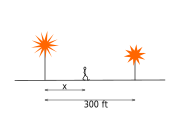
\includegraphics{05lamppost.pdf}}




The \textit{combined light intensity} is the sum of the two light
intensities coming from both lamp posts.




\subprob If you are in between the lamp posts, at distance $x$
feet from the stronger light, then give a formula for the combined light
intensity coming from both lamp posts as a function of $x$.




\subprob What is the darkest spot between the two lights, i.e.\
where is the combined light intensity the smallest?




\answer %{{{3
\textbf{(a)} The intensity at $x$ is a function of $x$.  Let's
call it $I(x)$.  Then at $x$ the distance to the big light is
$x$, and the distance to the smaller light is $1000-x$. Therefore
\[
  I(x) = \frac{1000}{x^2} + \frac{125}{(1000-x)^2}
\]
\textbf{(b)} Find the minimum of $I(x)$ for $0<x<1000$.
\[
  I'(x) = -2000 x^{-3} + 250(1000 - x)^{-3}.
\]
$I'(x) = 0$ has one solution, namely, $x= \frac{1000}{3}$.
By looking at the signs of $I'(x)$ you see that $I(x)$ must have a
minimum.  If you don't like looking at signs, you could instead
look at the second derivative
\[
  I''(x) = 6000 x^{-4} + 750 (1000 - x)^{-4}
\]
which is always positive.
\endanswer








\problem  %biggest soup can %{{{3
\subprob You have a sheet of metal with area $100\text{ in}^2$
from which you are to make a cylindrical soup can (with both a top and a bottom).  If $r$ is the
radius of the can and $h$ its height, then which $h$ and $r$ will
give you the can with the largest volume?
\answer %{{{3
The soup can is made of two disks (the top and bottom) and the side.
Both top and bottom have area $\pi r^2$.
The side can be made by bending a rectangular piece of metal into
a cylinder.  The sides of the rectangular piece of metal needed for
this are $h$ (height of the cylinder) and $2\pi r$ (perimeter of
the cylinder).  Therefore the total area of the metal that is needed
to make a cylinder of height $h$ and radius $r$ is
\[
A = 2\pi r^2 + 2\pi rh = 100 \mathsf{in}^2.
\]
The volume of that cylinder is
\[
V = \text{area base} \times \text{height} = \pi r^2h.
\]
We have to choose which variable we use to distinguish the different
sizes of cans that we can make.  The variables at hand are $r$
and $h$.  If we choose $h$ then we would have to get rid of $r$,
which involves solving the equation $A=100$ for $r$.  That equation
is quadratic, and formula for $r$ will involve square roots.




The other choice is the variable $r$.  Then we have to eliminate $h$,
i.e.~solve $A=100$ for $h$.  The solution is
\[
2\pi r^2 + 2\pi rh = 100 \implies
h = \frac{100 - 2\pi r^2} {2\pi r}.
\]




\endanswer




\subprob If instead of making a plain cylinder you replaced the
flat top and bottom of the cylinder with two hemispherical caps, then
(using the same 100in$^2$ of sheet metal), then which choice of
radius and height of the cylinder give you the container with the
largest volume?




\subprob Suppose you only replace the top of the cylinder with a
hemispherical cap, and leave the bottom flat.  Then which choice of height
and radius of the cylinder result in the largest volume?




\answer %{{{3
\textbf{(a)} The optimal radius is $r = \sqrt{50/3\pi}$, and the corresponding
height is $h = 100/(3\pi r) = 100/\sqrt{150\pi}$.
\endanswer





\problem A triangle has one vertex at the origin $O(0,0)$, another at the %{{{3
point $A(2a,0)$ and the third at $(a, a/(1+a^3))$.  What are the largest
and smallest areas this triangle can have if $0\leq a<\infty$?

\problem \groupproblem \textit{(Queen Dido's problem)} %{{{3

According to tradition Dido was the founder and first Queen of
Carthage.  When she arrived on the north coast of Africa
($\sim$800BC) the locals allowed her to take as much land as could be
enclosed with the hide of one ox.  She cut the hide into thin strips
and put these together to form a length of 100 yards\footnote{I made
that number up.  For the rest start at
\url{http://en.wikipedia.org/wiki/Dido}}.


    \begin{picture} (180.000000,48.725000)(0,0)
    \put(0.0, 0.0){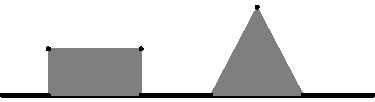
\includegraphics{05dido.pdf}}
        \put( 15.25,   6.22){\sffamily\itshape $A$}
    \put( 15.25,  28.48){\sffamily\itshape $B$}
    \put( 70.75,  28.48){\sffamily\itshape $C$}
    \put( 70.75,   6.22){\sffamily\itshape $D$}
    \put( 95.12,   6.22){\sffamily\itshape $P$}
    \put(126.38,  48.50){\sffamily\itshape $Q$}
    \put(148.62,   6.22){\sffamily\itshape $R$}
    \put(167.88,   6.22){\sffamily\itshape land}
    \put(167.88,  -6.78){\sffamily\itshape water}
\end{picture}


\subprob \rule{0pt}{14pt} If Dido wanted a rectangular region,
then how wide should she choose it to enclose as much area as
possible (the coastal edge of the boundary doesn't count, so in this
problem the length $AB+BC+CD$ is 100 yards.)

\subprob If Dido chose a region in the shape of an isosceles
triangle $PQR$, then how wide should she make it to maximize its area
(again, don't include the coast in the perimeter: $PQ+QR$ is 100
yards long, and $PQ=QR$.)


\problem The product of two numbers $x, y$ is 16. We know $x\geq 1$ and $y %{{{3
\geq1$. What is the greatest possible sum of the two numbers?


\problem What are the smallest and largest values that $(\sin x)(\sin y)$ can %{{{3
have if  $x+y=\pi$ and if $x$ and $y$ are both nonnegative?


\problem What are the smallest and largest values that $(\cos x)(\cos y)$ can %{{{3
have if  $x+y=\frac\pi2$ and if $x$ and $y$ are both nonnegative?


\problem %max&min of tan x+tan y, with x+y=pi/2 %{{{3
\subprob  Find the smallest and largest values of $\tan x
+ \tan y$ can have if $x+y=\frac\pi2$ and if $x$ and $y$ are both
nonnegative?




\subprob
What are the smallest and largest values that $\tan x + 2\tan y$ can
have if  $x+y=\frac\pi2$ and if $x$ and $y$ are both nonnegative?





\problem If a locomotive is traveling at $v$ miles per hour, the cost per hour %{{{3
of fuel $v^2 /25$ dollars, and other costs are \$100 per hour regardless of
speed. What is the speed that minimizes cost \textbf{per mile}?

\problem \groupproblem Josh is in need of coffee.  He has a circular filter with %{{{3
3 inch radius.  He cuts out a wedge and glues the two edges $AC$ and $BC$
together to make a conical filter to hold the ground coffee.  The volume $V$ of
the coffee cone depends the angle $\theta$ of the piece of filter paper Josh
made.

\centerline{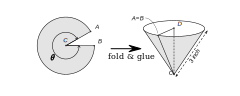
\includegraphics{05melita.pdf}}

\subprob  Find the volume in terms of the angle $\theta$.  (Hint:
how long is the  circular arc $AB$ on the left?  How long is the
circular top of the cone on the right?  If you know that you can find
the radius $AD=BD$ of the top of the cone, and also the height $CD$ of
the cone.)

\subprob Which angle $\theta$ maximizes the volume $V$?

\problem  Here are two equivalent problems (read both \& choose one): %{{{3

\subprob Blood pressure is the pressure exerted by circulating blood on
walls of the arteries. Assume the blood pressure varies periodically
according to the formula
\[
  p(t) = 50 +15\sin(2.5\pi t)
\]
where $t$ is the number of seconds since the beginning of a cardiac
cycle. When is the blood pressure the highest for $0 \leq t \leq 1$? What
is the maximum blood pressure? When is the blood pressure lowest in the
interval $0 \leq t \leq 1$ and what is the corresponding blood pressure?

\subprob The water level in a well is described as a function of time by
\[
  p(t) = 50 +15\sin(2.5\pi t).
\]
What is highest (resp.~smallest) water level in the time
interval $0 \leq t \leq 1$?








\problem A manufacturer needs to make a cylindrical can (with top and bottom) that will hold $1$ liter %{{{3
of liquid.  Determine the dimensions of the can that will minimize the amount of
material used in its construction.




\problem A window is being built in the shape of semicircle on the top of a %{{{3
rectangle, where there is a frame between the semicircle and rectangle as well
as around the boundary of the window. If there is a total of $15$ meters of
framing materials available, what must the dimensions of the window be to let in
the most light?

\problem A $5$ feet piece of wire is cut into two pieces. One piece is bent into %{{{3
a square and the other is bent into an equilateral triangle.  Where should the
wire be cut so that the total area enclosed by both figures is minimal?

\problem Two poles, one $5$ meters tall and one $10$ meters tall, are $20$ %{{{3
meters apart.  A telephone wire is attached to the top of each pole and it is
also staked to the ground somewhere between the two poles.

\subprob Where should the wire be staked so that the minimum amount of wire is
used?

\subprob Where should the wire be staked so that the angle formed by the two
pieces of wire at the stake is a maximum?


\problem Determine the cylinder with the largest volume that can be %{{{3
inscribed in a cone of height $10$ cm and base radius $6$ cm.



\problem A straight piece of wire $10$ feet long is bent into the shape of a %{{{3
right-angled $L$-shape. What is the shortest possible distance between the ends?

\problem An open-top cylindrical tank with a volume of $10$ cubic feet is to be %{{{3
made from a sheet of steel. Find the dimensions of the tank that will require as
little material used in the tank as possible.

\problem A box with a square base and open top must have a volume of $32,000$ %{{{3
  $\text{cm}^3$. Find the dimensions of the box that minimize the amount of material used
for building it.

\problem Find the length of the shortest ladder that will reach over an %{{{3
8-ft.~high fence to the wall of a tall building which is 3 ft.~behind the
fence.

\problem A rectangular piece of paper is 10 inches high and 6 inches %{{{3
wide. The lower right-hand corner is folded over so as to reach the
leftmost edge of the paper. Find the minimum length of the resulting
crease.




%%
%%\problem %{{{3
%%\begin{trivlist}
%%\item[(Bio)] The rate at which the body weight $y$ changes with respect to
%%  the age $x$ is proportional to $y^c$, for $c$ a species-specific positive
%%  constant. The relative growth rate defined as $\frac{1}{y} \cdot
%%  \frac{dy}{dx}$ measures the percentage weight gained per unit of
%%  time. For what values of $c$ is the relative growth rate increasing, and
%%  for which values it is decreasing?
%%\end{trivlist}
%%




%%\problem %{{{3
%%\begin{trivlist}
%%\item[(Bio)] The concentration of nitrogen in the soil is given by the
%%  function
%%  \[
%%  N(x)=(3-x)(4-x), \ \ \ 0 \leq x \leq 3
%%  \]
%%
%%  where $x$ is the depth in the soil where the measurement takes place.  At
%%  what depth from the soil surface is the concentration of nitrogen
%%  maximal?
%%\item[(Che)] The reaction rate of a chemical process is given by the
%%  function
%%  \[
%%  R(x)=(3-x)(4-x), \ \ \ 0 \leq x \leq 3
%%  \]
%%
%%  where $x$ is the concentration of the product resulted from the
%%  reaction. Find the concentration $x$ that maximizes the reaction rate.
%%
%%\item[(EMP)] A particle moving in the region of the plane given by $0 \leq
%%  x \leq 3$ follows a trajectory described by the equation
%%  $y(x)=x^2-7x+12$. Find the $x$-coordinate of the position of the particle
%%  corresponding to the highest $y$ coordinate.
%%\end{trivlist}
%%
\problem In the $xy$-plane, an observer stands at the origin $(0,0)$. A car %{{{3
travels along the curve $y=1/x^2$. How close does the car come to the observer?




%%\problem %{{{3
%%\begin{trivlist}
%%\item[(Bio)] The Pacific salmon can breed only once during its
%%  lifetime. The per capita rate of increase $r$ is a measure of
%%  reproductive fitness, in the sense that the greater $r$, the more
%%  offspring an individual produces. The rate of increase $r$ is a function
%%  of age $x$, given by
%%  \[
%%  r(x)=\frac{\ln[u(x)v(x)]}{x}
%%  \]
%%  where $u(x)$ is the probability of surviving to age $x$, and $v(x)$ is
%%  the number of female births at age $x$. Find the optimal age of
%%  reproduction, that is, the age $x$ that maximizes $r(x)$, if
%%  $u(x)=e^{-2x}$ and $v(x)=3x^2$.
%%\item[(EMP)] The efficiency of a technological process is measured by the
%%  function
%%  \[
%%  r(x)=\frac{\ln[3x^2e^{-2x}]}{x}
%%  \]
%%  where $x$ is the number of units produced. What number of units should be
%%  produced in order to maximize the efficiency function?
%%\end{trivlist}




%%\problem %{{{3
%%\begin{trivlist}
%%\item[(Bio)] The yield $y$ of an agricultural crop as a function of
%%  nitrogen level $x$ in the soil is modeled by the relationship
%%  \[
%%  y(x)=\frac{x}{1+x^2}, \ \ {\rm for} \ \ x \geq 0.
%%  \]
%%
%%  Find the nitrogen level that maximizes the yield.
%%\item[(Che)] The temperature $T$ in a certain chemical reaction varies as a
%%  function of time $t$ according to the rule
%%  \[
%%  T(t)=\frac{t}{1+t^2}.
%%  \]
%%  At what time during the reaction is the temperature at its maximal value?
%%\item[(EMP)] The pressure $P$ in a gas chamber varies as a function of time
%%  $t$ according to the rule
%%  \[
%%  P(t)=\frac{t}{1+t^2}.
%%  \]
%%  When is the pressure in the chamber at its highest value?
%%\end{trivlist}
%%
%%\problem ({\it van der Waals equation for real gases}) %{{{3
%%
%%The {\it ideal gas law} asserts that $PV=nRT$, where $P$ is the pressure
%%of the gas, $V$ is the gas volume, $n$ is the number of moles of gas, $T$
%%is the gas temperature, and $R$ is the ideal gas constant. However, the
%%ideal gas law does not hold at high pressures, and the {\it van der Waals
%%equation} for real gases
%%\[
%%  (P+\frac{n^2 a}{V^2})(V-nb)=nRT
%%\]
%%is used instead. The {\it van der Waals constants} $a$ and $b$ have been
%%determined experimentally for each gas. The {\it pressure deviation from
%%ideality}
%%\[
%%  P_{\rm dev}=P_{\rm real}-P_{\rm ideal}
%%\]
%%measures the difference in pressure as predicted by the ideal gas law, and,
%%respectively, van der Waals' law.
%%
%%$1.00$ mol of nitrogen N$_2$ is stored in a closed but flexible container
%%at a temperature of $300$ K.  What gas volume corresponds to the maximal
%%deviation from ideality $P_{\rm dev}$ if $R=0.08206$ $L \cdot
%%\textrm{atm}/\textrm{mol} \cdot
%%K$, $a=1.39$ $L^2 \cdot \textrm{atm}/\textrm{mol}^2$ and $b=0.0391$
%%$L/\textrm{mol}$?
\end{multicols}
\noproblemfont


\section{Parametrized Curves} %{{{1
\label{sec:05parametrized-curves-and-lHopital}
So far all the plane curves that we have seen were graphs of
functions $y=f(x)$.  A different way of describing a plane curve is to think of it as the
path that is traced out by a particle moving in the plane.  If you have a particle
that is moving about in the plane, then you can describe its motion by
specifying the coordinates $(x, y)$ of the point as functions of time: the
motion is given by two functions
\[
x = x(t), \quad y=y(t).
\]%
\marginpar{\input ../figures/221/05parametrized-curve.pdf_tex }%
As $t$ varies (``as time goes by'') the point $(x(t), y(t))$ traces out a curve.
This kind of curve is called a \emph{parametric curve} (or sometimes
\textit{parametrized curve}, or ``a curve defined by parametric equations'').
This topic reappears in third semester calculus (Math 234) where much of the
material can be simplified using vectors.




\subsection{Example: steady motion along a straight line} %{{{2
The simplest motion is where the particle moves with constant velocity.
Suppose the particle starts out at $(x_0, y_0)$ at time $t=0$, and
suppose its horizontal and vertical velocities are $v_x$ and $v_y$,
respectively.  Then after a time $t$ has gone by the point has moved a
distance $v_x t$ in the $x$-direction and $v_y t$ in the
$y$-direction.  Its coordinates are therefore
\begin{equation}
  x(t) = x_0 + v_x t, \quad
  y(t) = y_0 + v_y t.
  \label{eq:05motion-on-line}
\end{equation}
One question we can ask is: how fast is the particle moving?


\begin{figure}[h]
  \sffamily\small%
  \input ../figures/221/05motion-on-a-line.pdf_tex
  \caption{Motion with constant velocity along a straight line}
\end{figure}
We know that both its $x$-coordinate and $y$-coordinate increase at constant
rates $v_x$ and $v_y$.  So, between time $t$ and time $t+\Delta t$, the $x$ and
$y$ coordinates increase by $\Delta x = v_x \Delta t$ and $\Delta y =v_y \Delta
t$, so therefore the distance traveled by the point is
\begin{equation}
  \Delta s = \sqrt{(\Delta x)^2 + (\Delta y)^2} = t\,\sqrt{v_x^2 + v_y^2}.
  \label{eq:05distance-travelled-along-line}
\end{equation}
Then we can get the average speed $v$ by dividing by $\Delta t$:
\begin{equation}
  v = \frac{\Delta s} {\Delta t}
  = \sqrt{\Bigl(\frac{\Delta x}{\Delta t}\Bigr)^2
    + \Bigl(\frac{\Delta y}{\Delta t}\Bigr)^2}
  =\sqrt{v_x^2 + v_y^2}.
  \label{eq:velocity-along-line}
\end{equation}
Since the average speed turns out not to depend on the length $\Delta t$ of
the time interval, we see that the instantaneous speed at any time $t$
will also be equal to the value $v$ we have just found.


\begin{figure}[t]
  \small%
  \input ../figures/221/05motion-on-a-circle.pdf_tex
  \caption{\textbf{Constant velocity motion along a circle.}  The
    coordinates of any point on the circle with radius $R$ and center
    $(x_0,y_0)$ are completely determined by the angle $\theta$ (on
    the right).  To describe the motion of a particle on the circle you
    only have to specify how the angle $\theta$ changes with time.
    For a motion with constant angular velocity (on the left) $\theta$
    starts out at some value $\phi$ when $t=0$; after time $t$ the
    angle $\theta$ has increased by $\omega t$, and thus has the value
    $\theta = \phi+\omega t$. }
\end{figure}
\subsection{Example: steady motion along a circle} %{{{2
Suppose a particle $P$ is moving along a circle ``at a constant rate'',
or (to be more technical) ``with a constant angular velocity''.  Let the center
$C$ of the circle be at the point $(x_0, y_0)$ and let its radius be $R$.  The
location of $P$ is then completely determined by the angle $\theta$ that the
radius $CP$ makes with the horizontal line through the center; thus, we see that
the coordinates of $P$ are
\[
x = x_0 + R\cos \theta, \qquad y=y_0+R\sin \theta.
\]
Since the particle is moving on a circle, saying that it is moving at a constant rate is equivalent to saying that the angle $\theta$ is changing in time at a constant
rate.  This rate, usually called $\omega$, is the \emph{angular velocity} of the
point.  If the angle $\theta$ starts out at time $t=0$ with the value
$\theta=\phi$, then after time $t$ the angle $\theta$ has increased $\omega t$,
so that $\theta = \phi+\omega t$.  The motion of our particle $P$ is therefore
given by
\begin{equation}
  x(t) = x_0 + R\cos (\omega t + \phi), \quad
  y(t) = y_0 + R\sin (\omega t + \phi).
  \label{eq:05motion-on-circle}
\end{equation}
The initial angle $\phi$ is sometimes called the \emph{phase}.




\subsection{Example: motion on a graph} %{{{2
\label{sec:motion-on-a-graph}
\hangindent-170pt\hangafter-10\noindent%
If you are given a function $y=f(x)$ then we can describe its graph as a
parametric curve by setting
\[\displaywidth180pt
  x(t) = t \text{ and }y(t)= f(t).
\]
For this parametric curve we always have $y(t) = f(x(t))$ so the point with
coordinates $(x(t), y(t))$ always lies on the graph of the function $f$.
\centerline{\input ../figures/221/05motion-on-a-graph.pdf_tex }




Since $x(t) = t$ the point moves from left to right in such a way that its
horizontal velocity is $v_x=1$.




\subsection{General motion in the plane} %{{{2
In the most general motion of a point in the plane, the coordinates of the point
$P$ are given by two functions of time
\begin{equation}
  P:\quad x = x(t), \quad y = y(t).
  \label{eq:05motion-in-plane-in-general}
\end{equation}
In this course we mostly think of $t$ as ``time'' but the quantity $t$ doesn't
have to have that interpretation.  The important property of $t$ is that it is
a \emph{parameter} that allows us to label the points on the curve defined by
\eqref{eq:05motion-in-plane-in-general}.


To find the \emph{instantaneous velocity} of the point at some given time $t$
you follow the same strategy as in Chapter~\ref{ch:derivs1}.  Pick a (small)
number $\Delta t$ and compute the average velocity of the point between times
$t$ and $t+\Delta t$.  Then take the limit for $\Delta t\to 0$ to get the
instantaneous velocity.

Between time $t$ and time $t+\Delta t$ the $x$ and $y$ coordinates of the point
changed by $\Delta x$ and $\Delta y$, respectively, and therefore the average
velocities in the $x$ and $y$ directions are $\Delta x/\Delta t$ and $\Delta
y/\Delta t$.  The instantaneous horizontal and vertical velocities are
\[
v_x(t) = \lim_{\Delta t\to 0} \frac{\Delta x} {\Delta t} = \frac{dx}{dt},
\qquad
v_y(t) = \lim_{\Delta t\to 0} \frac{\Delta y} {\Delta t} = \frac{dy}{dt}.
\]
The distance traveled by the point from time $t$ to time $t+\Delta t$ is again
given by \eqref{eq:05distance-travelled-along-line}, i.e.~by $\Delta s =
\sqrt{(\Delta x)^2 + (\Delta y)^2}$.  Dividing by $\Delta t$, we find that the
average velocity between $t$ and $t+ \Delta t$ is
\[
\frac{\Delta s} {\Delta t}
=
\sqrt{\Bigl(\frac{\Delta x} {\Delta t}\Bigr)^2 +
  \Bigl(\frac{\Delta y} {\Delta t}\Bigr)^2}.
\]
Let $\Delta t\to 0$ to get the instantaneous velocity at time $t$:
\begin{equation}
  v(t) = \lim_{\Delta t\to 0} \frac{\Delta s} {\Delta t}
  =\sqrt{ \Bigl(\frac{dx} {dt} \Bigr)^2
    + \Bigl(\frac{d y} {dt}\Bigr)^2}
  =\sqrt{v_x(t)^2 + v_y(t)^2} \,.
  \label{eq:05instantaneous-velocity}
\end{equation}
\begin{figure}[t]\sffamily
  \input ../figures/221/05motion-on-a-curve2.pdf_tex
  \caption{Motion along a curve: the figure on the right, obtained by
    magnifying a small piece of the curve on the left, is almost, but
    not quite, a triangle.  It fails to be a triangle because the
    hypotenuse is not a straight line.  The smaller you make $\Delta
    t$, or, the closer you ``zoom in'' on the curve, the more the
    figure on the right will seem to be a right triangle.  This picture
    allows you to compute the velocity of the moving point $P$, and
    the slope $\tan \alpha$ of the tangent to the curve traced out by
    the point $P$ during this motion}
  \label{fig:05motion-along-a-curve}
\end{figure}
\subsection{Slope of the tangent line} %{{{2
In most examples the curve that gets traced out by $x=x(t)$, $y=y(t)$ has a
tangent line at most points.  To find the slope of that tangent line we follow the idea in
Chapter~II, \S\ref{sec:tangent}: first compute the slope of the line connecting two nearby
points on the curve and then consider the limit as the one of the two points
approaches the other.  More precisely, given a time $t$ choose a small time
increment $\Delta t\neq0$ and consider the points at times $t$ and $t+\Delta
t$. The slope of the line connecting these points is
\[
\text{Slope of secant} = \frac{\Delta y}{\Delta x}
\qquad
\text{(see Figure~\ref{fig:05motion-along-a-curve}).}
\]
To relate this to derivatives of $x(t)$ and $y(t)$ with respect to time we
rewrite this as
\[
\text{Slope of secant} = \frac{\Delta y}{\Delta x} = \frac{\dfrac{\Delta
    y}{\Delta t}}{\dfrac{\Delta x}{\Delta t}}
\]
Now we let $\Delta t\to 0$ and we find
\begin{equation}
  \text{Slope of tangent}
  = \lim_{\Delta t\to0}
  \frac{\;\dfrac{\Delta y}{\Delta t}\;}{\dfrac{\Delta x}{\Delta t}}
  =\frac{\;\dfrac{dy}{dt}\;}{\dfrac{dx}{dt}}
  =\frac{v_y(t)} {v_x(t)}.
  \label{eq:05slope-of-tangent-parametrized-curve}
\end{equation}
In Leibniz' notation this formula becomes very transparent: the slope of the
tangent to the curve is $dy/dx$, i.e.~the ratio of $dy$ and $dx$ where $dy$ is
the infinitely small increase of $y$ associated with an infinitely small
increase $dx$ of $x$.  If you pretend that infinitely small quantities exist,
then you can divide numerator and denominator in the fraction $dy/dx$ by $dt$,
which leads to
\[
\text{slope }= \frac{dy} {dx} = \frac{\;\dfrac{dy}{dt}\;}{\dfrac{dx} {dt}}.
\]
This same argument can also be given without referring to infinitely small
numbers, and by invoking the Chain Rule instead: if we think of $y$ as a
function of $x$ which is itself a function of $t$, then the Chain Rule says
\begin{equation*}
  \frac{dy}{dt} = \dfrac{dy}{dx} \cdot \dfrac{dx}{dt}
\end{equation*}
and now by rearranging we obtain the formula
\begin{equation*}
  \frac{dy}{dx} = \dfrac{dy/dt}{dx/dt} = \dfrac{y'(t)}{x'(t)}.
\end{equation*}


\subsection{The curvature of a curve} %{{{2
As the name says, curves are usually curved, and while they will touch
their tangent lines, a curve normally bends away from any tangent to
the curve.  Some curves appear more curved than others, while any
particular curve can be highly curved in some places and nearly
straight in others.

To make the phrase ``more curved'' more precise, you can compute the
\emph{curvature} of the curve at any given point.  The curvature
measures how fast the tangent to the curve is turning as you move
along the curve.  To define the curvature you first consider the angle
$\alpha$ that the tangent at any point on the curve makes with the
$x$-axis.  Given a point $P$ on the curve choose a nearby point $Q$
on the curve, and let $\Delta\alpha$ be the amount by which the
tangent angle changes as you go from $P$ to $Q$.  Then you could
define the ``average curvature'' of the segment $PQ$ to be the ratio
\[
\text{Average curvature of } PQ
= \frac{\Delta\alpha} {\Delta s},
\]
\marginpar{\input ../figures/221/05small-curved-arc.pdf_tex }%
where $\Delta s$ is the length of the arc $PQ$.  The \emph{curvature}
of the curve at the point $P$ is
\begin{equation}
  \kappa
  = \lim_{Q\to P}  \frac{\Delta\alpha} {\Delta s}.
  \label{eq:05curvature-def}
\end{equation}




\subsection{A formula for the curvature of a parametrized curve} %{{{2
\label{sec:formula-curvature-parametrized-curve}
How do you compute the limit \eqref{eq:05curvature-def} that defines
the curvature $\kappa$ if you know the functions $x(t), y(t)$ that specify the
parametric curve?




To compute $\kappa$ assume that the fixed point $P$ corresponds to a
certain value of $t$, so $P$ has coordinates $(x(t), y(t))$.  Let $Q$
be the point you get by changing $t$ to $t+\Delta t$, so $Q$ has
coordinates  $(x(t+\Delta t), y(t+\Delta t))$.  Then we get
\[
\kappa
= \lim_{Q\to P}  \frac{\Delta\alpha} {\Delta s}
= \lim_{\Delta t\to 0}
\frac{\dfrac{\Delta\alpha} {\Delta t}} {\dfrac{\Delta s} {\Delta t}}.
\]
The denominator is just the velocity
\[
\lim_{\Delta t\to 0} \dfrac{\Delta s} {\Delta t} = v = \sqrt{(x'(t))^2
+ (y'(t))^2}.
\]
The numerator is
\[
\lim_{\Delta t\to 0}
\frac{\Delta\alpha} {\Delta t} = \frac{d\alpha} {dt},
\]
i.e.,~it is the derivative of the tangent angle with respect to $t$
(time).  You can compute it by using
\[
\tan \alpha = \frac{y'(t)} {x'(t)}
\implies
\alpha = \arctan \frac{y'(t)} {x'(t)}.
\]
Using the chain rule and the quotient rule you can differentiate this
(a good exercise!), with result
\begin{equation}
  \frac{d\alpha} {dt} = \frac{x'(t)y''(t) - y'(t)x''(t)} {x'(t)^2
  + y'(t)^2}.
  \label{eq:05curvature-computation}
\end{equation}
To get the curvature we still have to divide by $v$.  The final result
is
\begin{equation}
  \kappa = \frac{x'(t)y''(t) - y'(t)x''(t)}
                {\bigl\{x'(t)^2 + y'(t)^2\bigr\}^{3/2}}.
  \label{eq:05curvature-of-parametrized-curve}
\end{equation}




\begin{figure}[ht]
  \centering \input ../figures/221/05radius-of-curvature.tex
  \caption{\textbf{The Osculating Circle and the Radius of
      Curvature. } If you assume that a small piece $PQ$ of a curve
    can be approximated by a circle, then this figure shows you how to
    compute the radius of that circle.  If the arc $PQ$ is a part of a
    circle with radius $R$, then the length $\Delta s$ of the arc is
    $R \Delta\alpha$, where $\gamma$ is the angle between the two
    normals to the arc at $P$ and $Q$.  The angle $\gamma$ is the same
    as the angle $\Delta \alpha$ between the two tangent lines to the
    curve at $P$ and $Q$.  The formula $\Delta s \approx R\Delta
    \alpha$ leads us to the definition $R = \lim_{Q\to P} \Delta
    s/\Delta\alpha$.}
  \label{fig:05osculating-circle}
\end{figure}




\subsection{The radius of curvature and the osculating circle} %{{{2
\label{sec:radius-curvature-osculating-circle}
Just as the tangent to a curve is the straight line that best approximates the
curve at some given point, you can try to find a circle that ``best
approximates'' the curve at some point.  This best match among all circles is
called the \emph{osculating circle} to the curve at the particular point.  Its
radius is the \emph{radius of curvature} of the curve.




For a more precise definition of the osculating circle, look at
Figure~\ref{fig:05osculating-circle}, which shows a curve with a point $P$.  To
find the circle through $P$ ``that best matches the curve'' we pick another
point $Q$ on the curve near $P$ and pretend that the arc $PQ$ is part of a
circle.  The center $C$ of the circle is then found by intersecting two normals
to the curve, one through $P$ and one through $Q$.  From basic geometry you know
that the length of a circular arc is the ``radius times the angle,'' so the
radius $R$ of the circle, the angle $\gamma$ between the normals, and the length
$\Delta s$ of the arc $PQ$ are related by
\[
\Delta s = R\times \gamma.
\]
Since you get the normals by rotating the tangents at $P$ and $Q$
counterclockwise by $90$ degrees, the angle $\gamma$ between the normals is the
same as the angle $\Delta \alpha$ between the tangents.  This leads to
\marginpar{\input ../figures/221/05computing-the-radius.pdf_tex }%
\[
R = \frac{\Delta s} {\Delta\alpha}.
\]
All this is based on the assumption that $PQ$ is a circular arc, but the curve
is not really a circle, and we should only expect the segment $PQ$ to be
\textit{approximately} a circle arc if the segment is ``short enough.''
Therefore we \textit{define} the radius of curvature to be the limit you get as
$Q\to P$:
\begin{equation}
  R  = \lim_{Q\to P} \frac{\Delta s} {\Delta\alpha}
  = \frac{1} {\lim_{Q\to P} \dfrac{\Delta\alpha} {\Delta s}}
  = \frac{1} {\kappa}.
\end{equation}
The \emph{osculating circle} at a point $P$ on a parametrized curve is
the circle with radius $R$ that is tangent to the curve at the point $P$.  The
center $C$ of the osculating circle lies on the normal to the curve at $P$.








\section{Problems} %{{{1
\problemfont %{{{3
\begin{multicols}{2}
\problem  Describe each of the following motions in the plane.  More %{{{3
specifically,  




\noindent
--find all points with a horizontal tangent,\\
--find all points with a vertical tangent,\\
--find all inflection points (i.e. points where the curvature $\kappa$ changes
sign).




\subprob \(x(t) =  1-t \), \(y(t) = 2- t  \)
\answer %{{{3
The straight line $y=x+1$, traversed from the top right to the bottom left
as $t$ increases from $-\infty$ to $+\infty$.
\endanswer




\subprob  \(x(t) =  3t+2 \), \(y(t) = 3t+2  \)
\answer %{{{3
The diagonal $y=x$ traversed from left to right.
\endanswer




\subprob  \(x(t) =  t \), \(y(t) = t^2  \)
\answer %{{{3
The standard parabola $y=x^2$, from left to right.
\endanswer




\subprob  \(x(t) =  \sin t \), \(y(t) = t  \)
\answer %{{{3
The graph $x=\sin y$.  This is the usual Sine graph, but on its side.




\centerline{\input ../figures/221/05vertical-sine-problem.tex }
\endanswer




\subprob  \(x(t) =  \sin t \), \(y(t) = \cos 2t  \)
\answer %{{{3
We remember that $\cos2\alpha = 1-2\sin^2\alpha$, so that
$x(t), y(t)$ traces out a part of the parabola $y=1-x^2$.
Looking at $x(t) = \sin t$ we see the point $(x(t), y(t))$ goes back
and forth on the part of the parabola $y=1-2x^2$ between $x=-1$
and $x=+1$.
\endanswer




\subprob  \(x(t) =  \sin 25t \), \(y(t) = \cos 25t  \)
\answer %{{{3
The unit circle, traversed \emph{clockwise}, 25 times every $2\pi$ time units.
Note that the angle $\theta = 25t$ is measured from the $y$-axis instead of from
the $x$-axis.




\begin{center}
  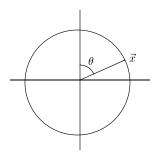
\includegraphics{05clockwise-circle-problem.pdf}
\end{center}
\endanswer




\subprob  \(x(t) =  1+\cos t \), \(y(t) = 1+\sin t  \)
\answer %{{{3
Circle with radius 1 and center $(1,1)$ (it touches the $x$ and $y$ axes).
Traversed infinitely often in counterclockwise fashion.
\begin{center}
  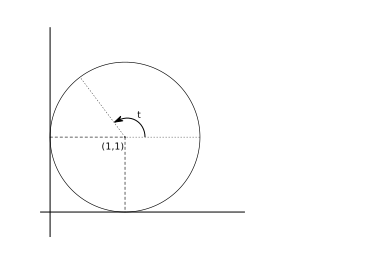
\includegraphics{05circle-at-1-1-problem.pdf}
\end{center}
\endanswer




\subprob  \(x(t) =  2\cos t \), \(y(t) = \sin t  \)
\answer %{{{3
Without the $2$ this would be the standard unit circle (dashed curve below).
Multiplying the $x$ component by $2$ stretches this circle to an ellipse.  So
$(x(t), y(t))$ traces out an ellipse, infinitely often, counterclockwise.




\begin{center}
  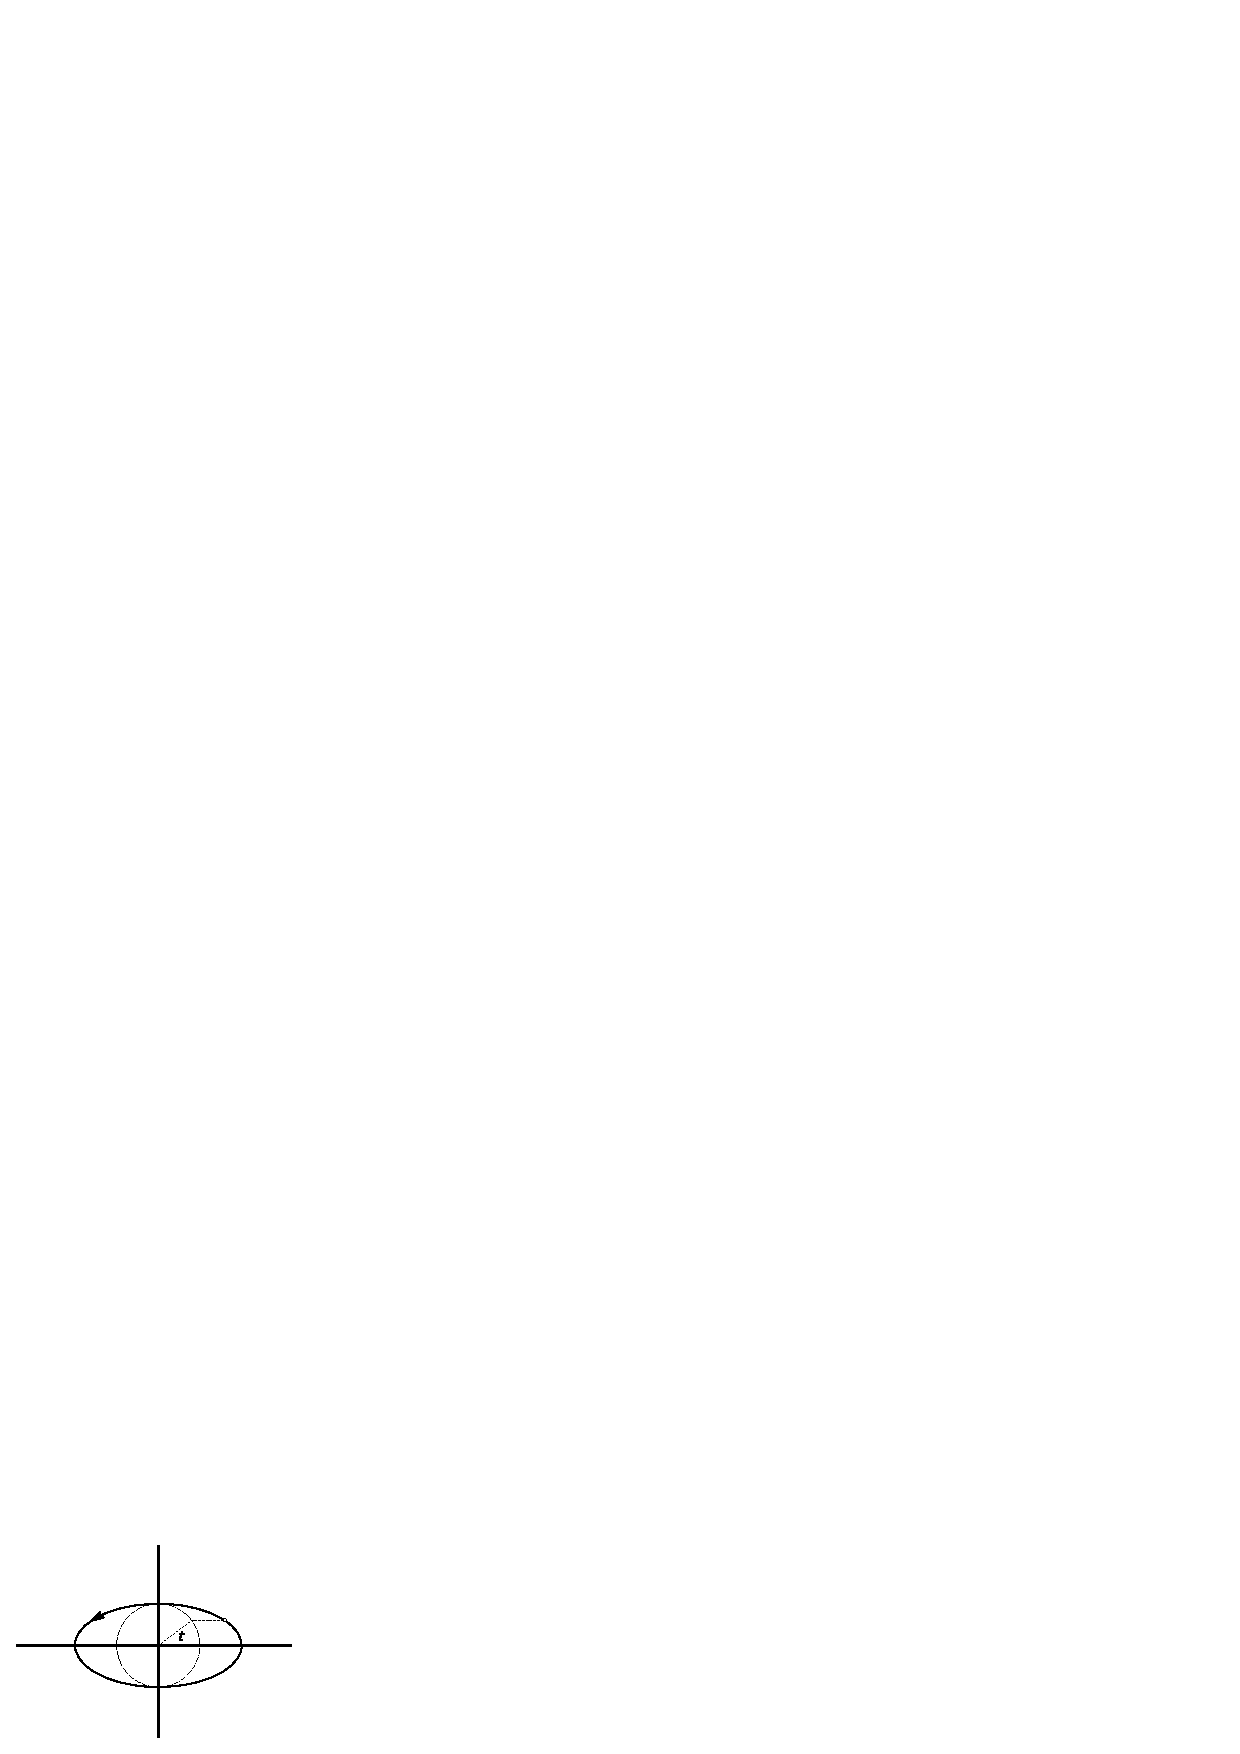
\includegraphics{05ellipse-problem.pdf}
\end{center}




\endanswer




\subprob  \(x(t) =  t^2 \), \(y(t) = t^3  \)
\answer %{{{3
For each $y=t^3$ there is exactly one $t$, namely, $t=y^{1/3}$.  So the curve is
a graph (with $x$ as a function of $y$ instead of the other way around).  It
is the graph of $x=y^{2/3} = \sqrt[3]{y^2}$.
\begin{center}
  \input ../figures/221/05neils-problem.tex
\end{center}
The curve is called \emph{Neil's parabola}.
\endanswer




\problem Complete the steps that led to \eqref{eq:05curvature-computation}. %{{{3




\problem Find the radius of curvature and the center of the osculating circle to %{{{3
the curve $x(t)=t, y(t) = 1/t$ at the point with $t=1$.




\problem  Find the curvature of the graph of a function $y=f(x)$.  You %{{{3
can do this be thinking of the graph of $y=f(x)$ as a parametric
curve as in \S~\ref{sec:motion-on-a-graph}, and then using
\eqref{eq:05curvature-of-parametrized-curve}.




The result you should get is
\[
\kappa = \frac{f''(x)} {\bigl(1+f'(x)^2\bigr)^{3/2}}\;.
\]




\problem Use the result from the previous problem to find points with the %{{{3
largest or smallest curvature on the following familiar graphs.  In each case
make a drawing of the graph first and guess your answer before you compute it.




\subprob Where is the curvature of the graph of $y=x^2$ largest?




\subprob Where is the curvature of the graph of $y=x^3$ largest?




\subprob Where is the curvature of the graph of $y=\frac13x^3$ largest?




\problem \carefulnow  Compute the curvature of the parametric curve given by %{{{3
$x(t) = \cos^2 t$, $y(t) = \sin^2 t$.




The answer turns out to be very simple and could have been predicted without
taking any derivatives -- do you see why?
\answer %{{{3
Since $\sin^2t + \cos^2 t =1$ we have $y(t) = 1-x(t)$ on this curve.  The curve
is a straight line and therefore its curvature is zero.
\endanswer




% \problem Consider the parametric curve %{{{3
% \[
%   x(t)=\frac{1-t^2}{1+t^2}, \quad y(t)=\frac{2t}{1+t^2}.
% \]
% \subprob Show that the curve traces out part of the unit circle.




% \subprob For which value of $t$ is $(x,y)=(1,0)$?  \; $(0,1)$?  $(0,-1)$? \;
% $\left(\frac35,\frac45\right)$?\;
% $\left(\frac{\sqrt{2}}{2},\frac{\sqrt{2}}{2}\right)$?\; Is there a value of $t$
% for which $(x,y)=(-1,0)$?












\end{multicols}
\noproblemfont




\section{l'Hopital's rule} %{{{1
\label{sec:05lhopitals-rule}




There is a simple way to compute limits of the form
\[
\lim_{t\to a} \frac{f(t)} {g(t)}
\]
that are of the form $\frac{0} {0}$, i.e.~where
\[
\lim_{t\to a} f(t) = 0
\text{ and }
\lim_{t\to a} g(t) = 0.
\]
It is given by what is called l'Hopital's rule, which says the
following:




\begin{theorem}
  If $f$ and $g$ both are differentiable functions such that 
  \[
    \lim_{t\to a} f(t) = 0 \text{ and } \lim_{t\to a} g(t) = 0,
  \]
  and if
  $\displaystyle \lim_{t\to a} \frac{f'(t)} {g'(t)}$ exists, then $\lim_{t\to a}
  \frac{f(t)} {g(t)} $ also exists.  Moreover,
  \[
    \lim_{t\to a} \frac{f(t)} {g(t)} = \lim_{t\to a} \frac{f'(t)} {g'(t)}
  \]
\end{theorem}\smallskip




\subsection{The reason why l'Hopital's rule works} %{{{2
\label{sec:reason-for-lHopital}
The two functions $f$ and $g$ define a parametric curve $x=g(t)$, $y=f(t)$
that is defined for $t\geq a$.  At $t=0$ we have $x=g(a) = 0$ and $y=g(a) = 0$,
so the origin lies on the curve traced out by $x=g(t)$, $y=f(t)$.




\noindent\rule{\textwidth}{1pt}\medskip




\def\mvtforlHopitalAnnotation
 {{\begin{minipage}{2.8in}\sffamily\itshape\footnotesize The slope of the chord
        connecting the origin and the point $(g(t), f(t))$ is
        \[\dfrac{f(t)}{g(t)}.\]

        Somewhere between this point and the origin there is a point $(g(c),
        f(c))$ on the curve where the tangent has the same slope. The slope of
        the tangent is
        \[\dfrac{f'(c)}{g'(c)}\]
      \end{minipage}
}}
\noindent%
\input ../figures/221/05mvt-for-lHopital2.pdf_tex%




\noindent\rule{\textwidth}{1pt}\smallskip

If we pick any value of $t>a$, then the ratio $\frac{f(t)} {g(t)}$ is the slope
of the chord connecting the two points $(0,0)$ and $(g(t), f(t))$ on the curve.
By the same kind of reasoning that led to the Mean Value Theorem (see Figure
\ref{fig:05MeanValueTheorem}) there has to be a point in between where the
tangent to the curve is parallel to the chord: in other words, there is some $c$
with $a<c<t$ such that
\[
\frac{f(t)} {g(t)} = \frac{f'(c)} {g'(c)}.
\]
The number $c$ depends on $t$, but since it lies between $a$ and $t$, we have
$\lim_{t\to a}c = a$.  
Therefore
\[
\lim_{t\to a}\frac{f(t)} {g(t)} = \lim_{c\to a}\frac{f'(c(t))} {g'(c(t))} =
\frac{f'(a)} {g'(a)}.
\]








 
\subsection{Examples of how to use l'Hopital's rule} %{{{2
The limit
\[
\lim_{x\to 1} \frac{3x^2-x-2} {x^2-1}
\]
is of the form $\frac{0} {0}$, so we can try to apply l'Hopital's rule.  We
get
\begin{equation}
\lim_{x\to 1} \frac{3x^2-x-2} {x^2-1}
=
\lim_{x\to 1} \frac{6x-1} {2x}
\label{eq:05lHopital-example1}
\end{equation}
So far we don't know if the limit exists, so it could be that we are
just saying that two things that don't exist are equal (whatever that
means).  But the second limit does exits:
\[
\lim_{x\to 1} \frac{6x-1} {2x} = \frac{6-1} {2} = \frac{5} {2}.
\]
Since this exists, l'Hopital's rule tells us that
the first limit in \eqref{eq:05lHopital-example1} also exists, and is
equal to $\frac52$.




For another example, consider the limit
\[
\lim_{x\to 0} \frac{\sin x} {x}
\]
which we have already computed in Chapter~III, \S\ref{sec:trigLimit}.  It is again
a limit of the form $\frac00$, so we can try to use l'Hopital's rule:
\[
\lim_{x\to 0} \frac{\sin x} {x} = \lim_{x\to0} \frac{\cos x} {1}
\stackrel{(*)}= \frac{1} {1} =1.
\]
The reasoning is that since the limit of $\dfrac{\cos x} {1}$ exists,
the limit of $\dfrac{\sin x}x$ must also exist and be the same.


Note that evaluating the limit $\lim_{x\to 0} \frac{\sin x} {x} = 1$ in this manner is actually circular reasoning, because we used this same limit in showing that the derivative of $\sin(x)$ is $\cos(x)$.


In the same way you can do a slightly more complicated example
\[
\lim_{x\to 0} \frac{\sin 5x} {\tan x}
=\text{``}\tfrac00\text{''}
\stackrel{\text{l'H}}=
\lim_{x\to0} \frac{5\cos 5x} {1/\cos^2x}
\stackrel{{(*)}}= \frac{5\cdot 1} {1/1^2} = 5.
\]
Again, the equality ``$\stackrel{\text{l'H}}=$''  follows from
l'Hopital's rule and the next equality ``$\stackrel{(*)}=$'' justifies
using the rule.




\subsection{Examples of repeated use of l'Hopital's rule} %{{{2
The limit
\[
\lim_{x\to 0} \frac {x - \sin x}{x^3}
\]
is again of the form $\frac00$.  When you apply l'Hopital's rule you
get
\[
\lim_{x\to 0} \frac {x - \sin x}{x^3}
=
\lim_{x\to 0} \frac {1 - \cos x}{3x^2},
\]
which is also of the form $\frac00$!  That means we can try to compute
this new limit by again applying l'Hopital's rule.  Here is the whole
computation:
\[
  \lim_{x\to 0} \frac {x - \sin x}{x^3}
  = \lim_{x\to 0} \frac {1 - \cos x}{3x^2}
  = \lim_{x\to 0} \frac {\sin x}{6x}
  = \lim_{x\to 0} \frac {\cos x}{6}
  = \tfrac16.
\]
Here we have applied l'Hopital's rule three times.  When we do this we
don't know if any of the limits that we run into actually exist, until
at the very end we find that the last limit exists (it's $\frac16$ in
this example).  The fact that the last limit exists implies that the
one before that exists; the fact the second to last limit exists in
turn implies that the limit before that one exists, and so on, until
we conclude that the limit we started with exists.  All the limits
must be equal, so we find that
\[
  \lim_{x\to 0} \frac {x - \sin x}{x^3} = \frac16,
\]
which means that for small values of $x$ we have the approximation
\[
x-\sin x \approx \tfrac16 x^3.
\]








\section{Problems} %{{{1
\problemfont %{{{3
\begin{multicols}{2}
\problem Compute the following limits using l'Hopital's rule. %{{{3




\subprob $\displaystyle \lim_{x\to 0} \frac{x^2-3} {x^2-8x-9}$.




\subprob $\displaystyle\lim_{x\to \pi/2} \frac{\sin 2x} {\cos x}$.




\subprob $\displaystyle\lim_{x\to 1/2} \frac{\cos \pi x} {1-2x}$.








\problem Suppose $n$ is some positive integer, and the limit %{{{3
\[
\lim_{x\to0} \frac{\cos x -1 -x^2/2} {x^n} = L
\]
exists. Also suppose $L\neq0$.
What is $n$?  What is the limit $L$?












\problem What happens when you use l'Hopital's rule to compute these %{{{3
limits?




\subprob $\displaystyle\lim_{x\to 0} \frac{x^2} {x}$.




\subprob $\displaystyle\lim_{x\to 0} \frac{x^2} {x^3}$.




\problem  Let $f(x) = \frac12x + x^2\sin\frac\pi x$ be the strange %{{{3
function whose graph is drawn in Figure
\ref{fig:05zigzagBetweenParabolas}.




\subprob Try to compute
\[
\lim_{x\to 0} \frac{f(x)} {x}
\]
in two ways:
\begin{itemize}
\item directly, and
\item by using l'Hopital's rule.
\end{itemize}




\subprob \carefulnow\carefulnow~~The following rule sounds very much
like l'Hopital's:
\begin{center}
  \itshape if $\displaystyle\lim_{x\to a} \frac{f(x)} {g(x)}$ exists,
  then $\displaystyle\lim_{x\to a} \frac{f'(x)} {g'(x)}$ also exists,
  and the two limits are equal.
\end{center}
But this is not always true!  Find a counterexample.








\problem Here is a method for computing derivatives: since, by %{{{3
definition,
\[
f'(a) = \lim_{x\to a} \frac{f(x) - f(a)} {x-a}
\]
is a limit of the form $\frac00$, we can always try to find it by
using l'Hopital's rule.  What happens when you do that?




\problem Simplicio did the following computation %{{{3
\begin{align*}
  \lim_{x\to 0} \frac{x} {\sin x}
  &= \lim_{x\to 0} \frac{1} {\cos x}\\
  &= \lim_{x\to 0} \frac{0}{\sin x}\\
  &= \lim_{x\to 0} 0\\
  &= 0\ldots?
\end{align*}
Do you see any problems with this?




\end{multicols}
\noproblemfont

%%% Local Variables:
%%% mode: latex
%%% TeX-master: "free221"
%%% End:
